\documentclass[12pt]{article}
\usepackage{report}
\usepackage{rotating}
\usepackage{tabularx}
\usepackage{booktabs}
\usepackage{float}
\usepackage{siunitx}
\usepackage{array}
\usepackage{titlesec}
\usepackage{tocloft}
% \usepackage{glossaries}
\usepackage[justification=centering]{caption}
\usepackage{booktabs}
\usepackage[table,xcdraw]{xcolor}
\usepackage{chngcntr}
\usepackage[utf8]{inputenc}
\usepackage{tabularx} % for better column control
\usepackage{caption}  % for table caption
\usepackage{booktabs} % for better table lines
\usepackage{enumitem}
\usepackage{multirow}  % For multirow table cells
\usepackage{xcolor}    % For colored cells (if not already loaded)

% Define Gantt chart symbols
\newcommand{\GantP}{\cellcolor{blue!30}P}      % Planning
\newcommand{\GantD}{\cellcolor{green!30}D}     % Development
\newcommand{\GantT}{\cellcolor{orange!30}T}    % Testing
\newcommand{\GantY}{\cellcolor{red!30}Y}       % Deployment
\newcommand{\GantC}{\cellcolor{gray!20}C}      % Continuous/Documentation

\usepackage[acronym]{glossaries}  % Load glossaries package
\makeglossaries  % Prepares glossaries for use

% Define acronyms (abbreviations)
\newacronym{cns}{CNS}{Central Nervous System}
\newacronym{mri}{MRI}{Magnetic Resonance Imaging}
\newacronym{cnn}{CNN}{Convolutional Neural Network}
\newacronym{vgg16}{VGG16}{Visual Geometry Group 16-layer model}
\newacronym{mern}{MERN}{MongoDB, Express.js, React.js, Node.js}
\newacronym{json}{JSON}{JavaScript Object Notation}
\newacronym{asr}{ASR}{Age-Standardized Rate}
\newacronym{relu}{ReLU}{Rectified Linear Unit}
\newacronym{ai}{AI}{Artificial Intelligence}
\newacronym{hmac}{HMAC}{Hash-based Message Authentication Code}
\newacronym{sha256}{SHA256}{Secure Hash Algorithm 256-bit}
\newacronym{rsa}{RSA}{Rivest–Shamir–Adleman}
\newacronym{jwt}{JWT}{JSON Web Token}


\title{Project proposal for BRAIN TUMOR ANALYSIS}
\author{Rohan Khanal}
\date{\today}

\begin{document}


{
\centering
\normalsize

\includegraphics[width=1.3in]{Images/TUlogo.png}\\

{TRIBHUVAN UNIVERSITY}\\
{INSTITUTE OF SCIENCE AND TECHNOLOGY}\\
CENTRAL CAMPUS OF TECHNOLOGY (CCT), HATTISAR, DHARAN
\\[1.5cm]
{\textit{A Internship Report On}\\
{\bf CLOUD AND DEVOPS ENGINEER }\\[1.5cm]

Submitted To:\\ DEPARTMENT OF IT \\ CENTRAL CAMPUS OF TECHNOLOGY (CCT),
HATTISAR, DHARAN, SUNSARI, KOSHI, NEPAL\\[1.5cm]

\textit{In partial fulfilment of the requirements for the degree of Bachelor's of Science in Computer Science and Information Technology  (B.Sc. CSIT)}\\[1.5cm]
% ~

Submitted By:\\{\bf ROHAN KHANAL} [29604/078]\\[0.5cm] {\bf TU Registration No} : 5-2-8-148-2021\\ [1.5cm]
% ~
Under the Supervision of:\\{\bf <Supervisor's Name>}\\[1.5cm]
Bhadra, 2082

}
}
%%% Local Variables:
%%% mode: plain-tex
%%% TeX-master: t
%%% End:
\thispagestyle{empty} 
\input{sec/coverpage} 
\thispagestyle{empty}

\newpage
\pagenumbering{roman}
\section*{\centering \Large \textbf{SUPERVISOR RECOMMENDATION}}
\addcontentsline{toc}{section}{Recommendation}
% \pagenumbering{roman} 
\sloppy
This is to recommend that \textbf{ROHAN KHANAL [29604/078]}, \textbf{DARSHAN DHAKAL [29592/078]}, and \textbf{SRIJAL BHATTARAI [29614/078]} have successfully carried out project work entitled ``\textbf{A CNN and Transfer Learning-Based MRI Brain Tumor Detection and Classification System}'' for the requirement of the project work in Bachelor of Science (B.Sc.) degree in CSIT under my supervision. This work was completed in the Department of IT, Central Campus of Technology, Institute of Science and Technology (IoST), Tribhuvan University (T.U.), Nepal.

% \vspace{1em}

To my knowledge, this work has not been submitted for any other degree. The students have fulfilled all the requirements laid down by the Institute of Science and Technology (IoST), Tribhuvan University (T.U.), Nepal for the submission of the project work for the partial fulfillment of Bachelor of Science (B.Sc.) degree in CSIT.

\begin{flushleft}
\begin{tabular}{@{}l@{}}
    \rule{4cm}{0.4pt} \\
    \textbf{Mr.\@ Prakash Neupane} \\
    \textbf{Supervisor} \\
    Department of IT \\
    Central Campus of Technology \\
    Hattisar, Dharan, Sunsari, Koshi, Nepal \\
\end{tabular}
\end{flushleft}

\newpage

\newpage
\section*{\centering \Large \textbf{DECLARATION}}
\addcontentsline{toc}{section}{Declaration}

\sloppy
This internship report, entitled ``{\bf DEVOPS}'', is being submitted to the Department of IT, Central Campus of Technology, Institute of Science and Technology (IoST), Tribhuvan University (T.U.), Nepal, for the partial fulfillment of the requirements for the Bachelor of Science (B.Sc.) degree in CSIT. This project has been carried out by us under the supervision of Prakash Neupane, T.U., Department of IT, Central Campus of Technology, Institute of Science and Technology (IoST), Tribhuvan University (T.U.), Nepal.

We hereby declare that this work is original and has not been submitted earlier, in part or in full, to this or any other university or institution, here or elsewhere, for the award of any degree.

\begin{flushleft}
\begin{tabular}{@{}l@{}}
    \textbf{ROHAN KHANAL [29604/078]} \\
    Department of IT \\
    Central Campus of Technology \\
    Hattisar, Dharan, Sunsari, Koshi, Nepal \\
\end{tabular}
\end{flushleft}

\newpage

\newpage
\section*{\centering \Large \textbf{CERTIFICATE OF APPROVAL}}
\addcontentsline{toc}{section}{Certificate of Approval}

This is to certify that the internship report entitled ``{\bf DEVOPS }'', submitted by {\bf Mr\@.\@ ROHAN
        KHANAL [29604/078]}, a student enrolled in the Bachelor of Science (B.Sc.) degree in CSIT at the Central Campus of Technology, Dharan, has been examined and approved by the undersigned.

The report has been evaluated based on its relevance to the internship experience, presentation of facts, adherence to prescribed guidelines, and overall quality. It has been found to meet the standards set by Tribhuvan University for the partial fulfillment of the requirements for the bachelor’s degree.\vspace{2cm}

\noindent
\begin{minipage}[t]{0.45\textwidth}
    \centering
    \rule{5cm}{0.4pt} \\
    \textbf{Mr.\@ Prakash Neupane} \\
    {\bf Supervisor}\\
    Department of IT\\
    Central Campus of Technology\\
    IOST, Tribhuvan University\\[3em]

    % $\overline{\text{{\bf External Examiner}}}$\\
    \vspace{1.5cm}
    \rule{5cm}{0.4pt} \\
    {\bf Mr.\@ Pradip Khatiwada} \\
    \textbf{External Examiner} \\
    Mechi Multiple Campus\\
    IOST, Tribhuvan University\\[3em]
\end{minipage}
\hfill
\begin{minipage}[t]{0.45\textwidth}
    \centering
    % $\overline{\text{{\bf Name of Program Director/HOD}}}$\\
    \rule{6cm}{0.4pt} \\
    \textbf{Mr.\@ Balabhadra Bhandari} \\
    {\bf Program Director}\\
    Department of IT\\
    Central Campus of Technology\\
    IOST, Tribhuvan University\\[3em]
\end{minipage}

\newpage


\newpage

\section*{\Large\centering \textbf{ACKNOWLEDGEMENT}}
\addcontentsline{toc}{section}{Acknowledgement}
We would like to express our heartfelt gratitude to \textbf{Mr.\@ Prakash Neupane}, our esteemed supervisor, whose invaluable guidance, unwavering support, and insightful feedback have been crucial to the successful completion of this project. His expertise and encouragement have been a constant source of motivation throughout the research, development, and implementation phases.\\[0.5em]
Our sincere appreciation also extends to all faculty members of the Central Campus of Technology for their guidance, inspiration, and constructive feedback, which have been instrumental in shaping our project.\\[0.5em]
Finally, we express our deepest gratitude to our families and friends for
their unwavering support, patience, and encouragement, which have been our strength
throughout this journey. Their belief in our abilities has inspired us to persevere and
complete this project successfully.\\[0.5em]
Thank you.

\begin{flushright}
    \begin{tabular}{l}
        \textbf{DARSHAN DHAKAL [29592/078]}   \\
        \textbf{ROHAN KHANAL [29604/078]}     \\
        \textbf{SRIJAL BHATTARAI [29614/078]} \\
    \end{tabular}
\end{flushright}

\newpage

\newpage
\section*{\Large\centering \textbf{ABSTRACT}}
\addcontentsline{toc}{section}{Abstract}
This report presents the design, development, and implementation of a comprehensive web-based brain tumor detection system utilizing deep learning techniques for medical image analysis. The system integrates a convolutional neural network (CNN) model with a modern full-stack web application to provide automated classification of brain tumors from MRI scans. The application distinguishes between four categories: Glioma, Meningioma, Pituitary tumors, and Normal brain scans. Built using React.js for the frontend, Node.js/Express.js for the backend, and TensorFlow/Keras for machine learning implementation, the system demonstrates the practical application of artificial intelligence in healthcare diagnostics. The system achieves high accuracy in tumor classification while providing a user-friendly interface for medical professionals and researchers. This work contributes to the growing field of computer-aided diagnosis (CAD) systems and demonstrates the potential of web-based AI applications in medical imaging.

% \hfill \vspace{1cm} \break 
\small
\noindent \textbf{\textit{Keywords:}} Brain tumor detection, Computer-aided diagnosis, Convolutional Neural Networks, Deep learning, Medical image analysis, MRI scans, Transfer learning, Web application.
\newpage

% Table of contents
\newpage
{
  \setlength{\parskip}{0em}
  \renewcommand{\contentsname}{}
  \section*{\Large\centering \textbf{CONTENTS}}
  \tableofcontents
}

% List of Abbreviations - if any
\newpage
\section*{\Large\centering \textbf{LIST OF ABBREVIATIONS}}
\printglossary[type=\acronymtype, title=]
\addcontentsline{toc}{section}{List of Abbreviations}




% List of figures - if any
\newpage
{
  \renewcommand{\listfigurename}{}
  \section*{\Large\centering \textbf{LIST OF FIGURES}}
  \listoffigures
  \addcontentsline{toc}{section}{List of Figures}
}

\newpage
{
  \renewcommand{\listtablename}{}
  \section*{\Large\centering \textbf{LIST OF TABLES}}
  \listoftables
  \addcontentsline{toc}{section}{List of Tables}
}

\newpage
\pagenumbering{arabic}

\section*{\Large\centering \textbf{CHAPTER 1 \\ INTRODUCTION }}
\addcontentsline{toc}{section}{CHAPTER 1: Introduction}
\setcounter{section}{1}

\subsection{Introduction}
In recent years, the software development industry has undergone a major transformation with the emergence of DevOps practices and Cloud Computing technologies. Traditional software development methodologies often separated development and operations teams, resulting in slow delivery cycles, frequent deployment failures, infrastructure inconsistencies, and limited scalability. To address these challenges, DevOps has emerged as a cultural and technical movement that integrates development (Dev) and operations (Ops) into a unified workflow, promoting automation, collaboration, continuous integration, and continuous delivery. \cite{HARNESSING_CLOUD_INFRASTRUCTURE}

DevOps is not merely a toolset but a philosophy that emphasizes automation, monitoring, version control, infrastructure as code (IaC), containerization, and cloud-based deployment. Combined with cloud computing platforms such as Amazon Web Services (AWS), DevOps enables organizations to build scalable, resilient, and highly available systems with faster release cycles and improved reliability. \cite{CI/CD}

During my internship at Genese Solution Pvt. Ltd., Lalitpur, Nepal, I worked as a Cloud and DevOps Engineering Intern, where I gained hands-on experience in implementing DevOps practices within real-world production environments. The organization specializes in cloud-based infrastructure solutions, automation, and scalable system design. Throughout the internship period, I was actively involved in designing and implementing CI/CD pipelines, managing AWS resources, automating deployment processes using AWS SAM (Serverless Application Model), configuring IAM roles and policies, and working with services such as AWS Lambda, CodeBuild, CodePipeline, S3, CloudFormation, EventBridge, and CloudWatch.

One of the major projects I contributed to involved a serverless architecture using AWS Lambda in a monorepo structure, where multiple independent Lambda functions shared common layers. The deployment was automated through CodePipeline and CodeBuild, enabling efficient version control and environment-based deployment (Development, Staging, Production). This experience provided deep practical exposure to infrastructure automation, cloud security, monitoring, and performance optimization.

This internship bridged the gap between academic learning and industry practices. It enhanced my understanding of distributed systems, cloud-native architectures, DevOps lifecycle, security best practices, and automation techniques required for modern software delivery.

\subsection{Problem Statement}
In traditional software development environments, several critical challenges exist:
\begin{itemize}
  \item Manual deployment processes leading to human errors
  \item Lack of standardized infrastructure configuration
  \item Poor collaboration between development and operations teams
  \item Inconsistent environments (development vs.\ production mismatch)
  \item Slow release cycles
  \item Difficulty in scaling applications
  \item Limited monitoring and observability
\end{itemize}

Organizations aiming to build cloud-based applications often struggle with:
\begin{itemize}
  \item Automating deployments efficiently
  \item Managing infrastructure securely
  \item Maintaining environment consistency
  \item Implementing continuous integration and continuous deployment (CI/CD)
  \item Managing multiple microservices or serverless functions efficiently
  \item Ensuring security and least-privilege access using IAM policies
\end{itemize}

Specifically, in serverless monorepo architectures, challenges arise in:
\begin{itemize}
  \item Handling shared dependencies (common layers)
  \item Triggering selective deployments
  \item Avoiding unnecessary rebuilds
  \item Maintaining version control for multiple Lambda functions
  \item Ensuring proper role-based access control
  \item Managing S3 artifacts and CloudFormation packaging
\end{itemize}

Therefore, there was a need to design and implement a structured DevOps workflow that would:
\begin{itemize}
  \item Automate build, package, and deployment processes
  \item Enable scalable serverless architecture
  \item Reduce manual intervention
  \item Improve deployment reliability
  \item Enforce security best practices
  \item Optimize cloud resource usage
\end{itemize}

% \subsection{Objectives}
%  To design and implement a convolutional neural network (\gls{cnn}) model, incorporating transfer learning with VGG16 to enhance accuracy, tailored for precise brain tumor detection and classification.

\subsection{Objectives}
To understand and implement DevOps practices using cloud technologies in a production-level environment.
% \begin{itemize}
%     \item To design and implement a convolutional neural network (\gls{cnn}) model.
%     \item To incorporate transfer learning with VGG16 to enhance accuracy for precise brain tumor detection and classification.
% \end{itemize}

\subsection{Scope and Limitation}
\textbf{Scope}
The scope of this internship primarily covered:
\begin{itemize}
  \item Implementation of DevOps practices in cloud-based environments
  \item Serverless architecture design using AWS Lambda
  \item CI/CD pipeline development
  \item Infrastructure as Code using AWS SAM and CloudFormation
  \item Cloud security configuration using IAM
  \item S3 artifact management
  \item Monitoring and logging setup
  \item Automation of multi-environment deployments
  \item Version control integration with Git repositories
\end{itemize}

The internship provided exposure to real-time production systems and enterprise-level deployment strategies. The practical implementation helped understand how scalable and reliable cloud architectures are built in modern organizations.

Furthermore, the internship experience is highly relevant to academic subjects such as:
\begin{itemize}
  \item Distributed Systems
  \item Cloud Computing
  \item Operating Systems
  \item Database Systems
  \item Software Engineering
  \item Computer Networks
\end{itemize}

\textbf{Limitation}
Despite the extensive exposure, certain limitations were present:
\begin{itemize}
  \item Limited access to confidential production data
  \item Restricted IAM permissions due to security policies
  \item Time-bound internship duration (12 weeks)
  \item Dependency on organizational infrastructure decisions
  \item Limited exposure to on-premises DevOps environments
  \item Focus primarily on AWS (not multi-cloud platforms)
\end{itemize}

Additionally, some enterprise-level configurations (e.g., advanced security compliance, cost governance strategies, and enterprise networking design) were outside the scope of the internship.


\subsection{Report Organization}
This internship report is organized into multiple chapters to systematically present the learning experience and technical contributions made during the internship.
\begin{itemize}
  \item \textbf{Chapter 1: Introduction} \\
  Provides background, objectives, problem statement, scope, and structure of the report.

  \item \textbf{Chapter 2: Organization Overview} \\
  Describes Genese Solution Pvt.\ Ltd., its services, working environment, and organizational structure.

  \item \textbf{Chapter 3: Literature Review / Background Study} \\
  Covers theoretical concepts related to DevOps, CI/CD, Cloud Computing, AWS services, Infrastructure as Code, and Serverless Architecture.

  \item \textbf{Chapter 4: Methodology and Tools Used} \\
  Explains the technologies, tools, and workflow implemented during the internship.

  \item \textbf{Chapter 5: System Design and Implementation} \\
  Describes the architecture, CI/CD pipelines, serverless deployment structure, IAM configuration, and automation strategies.

  \item \textbf{Chapter 6: Results and Discussion} \\
  Analyzes implementation outcomes, performance improvements, challenges faced, and solutions applied.

  \item \textbf{Chapter 7: Conclusion and Future Recommendations} \\
  Summarizes key learning outcomes and suggests possible improvements and future enhancements.

  \item \textbf{Appendices} \\
  Includes screenshots, configuration files, code snippets, pipeline diagrams, and additional documentation.
\end{itemize} % Ensure this file exists and is correctly formatted
% \pagenumbering{arabic}

\newpage
\section*{\Large\centering \textbf{ CHAPTER 2 \\ ORGANIZATION DETAILS AND LITERATURE REVIEW }}
\addcontentsline{toc}{section}{CHAPTER 2: Organization Details and Literature Review}
\setcounter{section}{2}
\setcounter{subsection}{0}

\subsection{Introduction to Organization}
Genese Solution Pvt. Ltd. is a multinational technology consulting and cloud services company with a strong presence in Nepal and several other countries across Europe and Asia. It operates as part of the larger Genese Solution group headquartered in the United Kingdom, offering a wide range of digital transformation solutions including cloud computing consultation, software development, cybersecurity, infrastructure automation, and DevOps services. The company specializes in helping organizations optimize their IT operations by leveraging modern cloud technologies such as Amazon Web Services (AWS), Microsoft Azure, and Google Cloud Platform to build scalable, secure, and cost-efficient systems. With a focus on innovation and customer-centric solutions, Genese Solution works with enterprises, startups, and public sector clients to design and deploy end-to-end digital solutions tailored to their unique business needs. \cite{genese_official_website}

In Nepal, Genese Solution has established itself as a key player in the IT and cloud consulting landscape, operating out of Jhamsikhel, Lalitpur and contributing significantly to the adoption of modern cloud and DevOps practices within the region. The company’s team comprises highly skilled and internationally certified professionals who bring deep technical expertise to projects involving cloud migration, DevOps automation, continuous integration and delivery (CI/CD), and infrastructure optimization. Through its services, Genese Solution helps organizations enhance operational efficiency, reduce manual intervention, and accelerate software delivery cycles. Additionally, the company engages in initiatives aimed at bridging the skill gap between academia and industry by supporting cloud education and workforce development, further strengthening Nepal’s technology ecosystem. \cite{genese_official_website}
\subsection{Organizational Hierarchy}
\subsection{Working Domains of Organization}

Genese Solution operates across multiple technology and consulting domains with a focus on enabling digital transformation and cloud adoption for businesses of all sizes. The primary working domains of the organization include:\

\begin{itemize}
    \item \textbf{Cloud Consulting \& Cloud Services:} Providing strategy, planning, migration, managed support, and optimization of cloud infrastructure, helping organizations transition to scalable and cost-efficient cloud platforms. 

    \item \textbf{DevOps and Cloud Automation:} Implementing modern DevOps practices including continuous integration and continuous deployment (CI/CD), infrastructure as code (IaC), automated deployment pipelines, monitoring, and operational automation. 

    \item \textbf{Software and Application Development:} Delivering web and mobile application solutions, backend systems, API development, and customized software to support business digitalization.

    \item \textbf{Cybersecurity \& Compliance Solutions:} Offering security assessments, compliance audits, cyber risk mitigation strategies, and secure architecture services to protect critical systems. 

    \item \textbf{Productivity \& Collaboration Tools:} Deployment and support of communication and productivity systems for enterprises, such as unified collaboration suites and monitoring tools.

    \item \textbf{Digital Marketing \& SEO Services:} Helping businesses improve online presence and engagement through search engine optimization and digital marketing strategies. 

    \item \textbf{Cloud Education \& Skill Development (Genese Cloud Academy):} Training programs and mentorship aimed at bridging the gap between academic knowledge and industry requirements by equipping students and professionals with cloud computing and DevOps skills.

    \item \textbf{Domain and Web Hosting Services:} Providing domain registration, hosting solutions, and managed server environments tailored to business needs.

    \item \textbf{Monitoring and Performance Optimization:} Tools and services dedicated to monitoring infrastructure performance, identifying anomalies, and optimizing cloud resource usage.
\end{itemize}

The organization’s expertise spans a wide spectrum of digital technology domains, enabling it to support clients across different industries by delivering secure, scalable, and future-ready technology solutions.

\subsection{Description of Intern Department}
During my internship at Genese Solution Pvt. Ltd., Nepal, I was placed within the Cloud \& DevOps Engineering Department, a core technical division responsible for implementing automation, cloud infrastructure solutions, and modern software delivery processes. This department plays a pivotal role in transforming how the company and its clients manage software deployment, infrastructure provisioning, and operational scalability. It focuses on designing, deploying, and maintaining cloud-native systems primarily on Amazon Web Services (AWS), as well as integrating continuous integration and continuous delivery (CI/CD) pipelines to streamline the development lifecycle. The team works collaboratively with cross-functional stakeholders to ensure production-grade automation, robust security practices, and highly available cloud architectures, all of which contribute directly to modern digital transformation goals.

\subsection{Literature Review}

DevOps is a modern software engineering paradigm that emerged to address the inefficiencies and disconnects between traditional software development and IT operations. At its core, DevOps emphasizes collaboration, shared responsibility, and continuous processes that span from initial code development to production deployment and operational monitoring. Studies define DevOps as a cultural and technical approach that integrates development and operations teams to improve software delivery performance while reducing errors and lead time for changes. DevOps adoption involves organizational transformation as much as technical change, requiring clear practices, guidelines, and close alignment of cross-functional teams to realize its full potential. Research has shown that adopting DevOps practices can significantly streamline processes, improve communication, and enhance overall software delivery quality and velocity. \cite{EXPLORING_THE_BENEFITS}

A foundational element of DevOps is the implementation of continuous practices such as Continuous Integration (CI) and Continuous Delivery/Deployment (CD). CI involves the frequent integration of code changes into a shared repository, triggering automated builds and tests to detect issues early in the software lifecycle. CD extends CI by automating the release and deployment of validated changes to production environments with minimal manual intervention, improving delivery speed and system reliability. Research in this area highlights that CI/CD pipelines reduce human errors, accelerate feedback loops, and support faster feature deliveries, which are critical for competitive advantage in today’s software-driven markets.\cite{CI/CD}

The role of cloud computing has become particularly significant in enabling DevOps practices at scale. The elasticity, automation, and on-demand infrastructure of cloud platforms provide ideal underpinnings for DevOps workflows, allowing teams to dynamically provision resources, scale testing environments, and manage releases across multiple environments. Cloud-enabled DevOps has been linked with higher deployment frequency, improved scalability, and better resource utilization. Nevertheless, literature also notes that the integration of cloud infrastructure within DevOps introduces new challenges related to security, cost management, and the handling of legacy systems, indicating that organizations must adopt structured strategies to address these concerns.\cite{HARNESSING_CLOUD_INFRASTRUCTURE}

Another critical practice within DevOps is Infrastructure as Code (IaC), which describes the automation of infrastructure provisioning and configuration through code rather than manual processes. IaC improves consistency, repeatability, and traceability of infrastructure changes, helping teams manage complex environments reliably.This aligns with modern DevOps objectives of automating as much of the software delivery lifecycle as possible, further enabling rapid, scalable deployments. \cite{aws_iac_whitepaper}

\newpage
\stepcounter{section}
\section*{\Large\centering {CHAPTER 3 \\ INTERNSHIP ACTIVITIES}}
\addcontentsline{toc}{section}{CHAPTER 3: Internship Activities}\label{3}

\subsection{Roles and Responsibilities}
\begin{enumerate}[label=\roman*.]
    \item \textbf{Functional Requirements}
          \begin{center}
              \begin{figure}[H]
                  \centering
                  \includegraphics[width=0.85\linewidth]{Images/usecase.pdf}
                  \caption{Use Case Diagram}
                  \label{fig:UseCaseDiagram}
              \end{figure}
          \end{center}
          The use case diagram presents the fundamental interactions between system actors and core functionalities of the application. The primary actor, Patient/User, represents individuals seeking brain tumor analysis services and can perform essential activities including account registration, system login, brain scan upload, image analysis, result viewing, report generation, profile management, analysis history review, and system logout. The diagram establishes key relationships through include and extend dependencies, where uploading brain scans necessarily includes the analysis process, viewing results can optionally extend to report generation, and successful login enables access to upload functionality.

    \item \textbf{Non-Functional Requirements}
          \begin{itemize}
              \item \textbf{Performance:} The system should process MRI images and provide classification results within 10--15 seconds per image, ensuring minimal waiting time for medical practitioners during diagnosis.

              \item \textbf{Accuracy:} The brain tumor classification model must maintain a minimum accuracy of 95\% on test datasets, with precision and recall rates above 90\% for each tumor type (glioma, meningioma, pituitary).

              \item \textbf{Usability:} The user interface must be intuitive and easy to navigate for medical practitioners with varying levels of technical expertise, requiring minimal training for effective system usage.

              \item \textbf{Reliability:} The system should maintain 99.5\% uptime with robust error handling and recovery mechanisms to ensure continuous availability for critical medical applications.

              \item \textbf{Security:} Patient data and medical images must be encrypted during transmission and storage, with secure user authentication to comply with healthcare data protection regulations.

              \item \textbf{Compatibility:} The web-based interface must be compatible with major browsers (Chrome, Firefox, Safari, Edge) and responsive across desktop, tablet, and mobile devices.

              \item \textbf{Maintainability:} The codebase should follow clean coding practices and modular design principles to facilitate future updates, model improvements, and feature additions.

              \item \textbf{Data Integrity:} The system must ensure data consistency and prevent corruption during image upload, processing, and storage operations with appropriate backup and recovery mechanisms.

              \item \textbf{Extensibility:} The system architecture should support future enhancements such as additional imaging modalities (CT scans, X-rays), new tumor types, and integration with existing hospital information systems.
          \end{itemize}

\end{enumerate}
\subsection{Weekly log}
\begin{enumerate}[label=\roman*.]
    \item \textbf{Technical} \\
          The system demonstrates strong technical viability through proven technology integration. The architecture combines React/TypeScript frontend with Node.js/Express backend, providing robust scalability for medical applications. TensorFlow/Keras implementation ensures reliable deep learning capabilities with 90\% accuracy in brain tumor classification. Docker containerization enables consistent deployment across environments, while MongoDB offers flexible medical data storage. JWT authentication and bcrypt encryption meet healthcare security standards. The system supports cross-platform compatibility and future DICOM integration, confirming technical robustness and extensibility for medical imaging workflows.

    \item \textbf{Operational} \\
          The system aligns effectively with existing healthcare workflows and user requirements. The intuitive web-based interface requires minimal training for medical professionals, supporting multiple user roles including patients, doctors, and administrators. Automated analysis reduces interpretation time while maintaining human oversight through confidence scoring. The system integrates seamlessly with existing radiology workflows and generates comprehensive PDF reports for documentation. Cloud deployment supports telemedicine scenarios, while flexible architecture accommodates both individual practitioners and institutional deployments across various healthcare settings.
    \item \textbf{Economic} \\
          The project demonstrates favorable cost-benefit ratios through open-source technology utilization, eliminating expensive licensing fees. Development costs remain manageable with estimated ROI within 18--24 months based on subscription models and pay-per-analysis pricing. The system addresses significant market demand for affordable medical imaging tools, particularly in resource-limited settings. Operational costs scale proportionally with adoption, while revenue potential exists through institutional subscriptions and premium features. Long-term sustainability benefits from cloud scaling and automated operations reducing maintenance overhead.

    \item \textbf{Schedule}
          The four-month development timeline from Jestha through Bhadra provides realistic project completion within allocated resources. Modular architecture enables parallel development streams, while agile methodology ensures continuous progress monitoring. The schedule accommodates comprehensive testing phases and risk mitigation strategies with adequate buffer time for unforeseen challenges. Critical milestones include system design completion, core functionality implementation, thorough testing, and final deployment preparation, ensuring successful delivery within the specified timeframe.
        %   \begin{figure}[H]
        %       \centering
        %       \includegraphics[width=1\linewidth]{Images/gantt.png}
        %       \caption{Sample Gantt Chart demonstrating schedule feasibility}
        %       \label{fig:gantt}
        %   \end{figure}

        \begin{table}[h!]
\centering
\footnotesize
\setlength{\tabcolsep}{2pt}
\resizebox{\textwidth}{!}{%
\begin{tabular}{@{}l*{16}{c}@{}}
\toprule
\multirow{2}{*}{\textbf{Task}} &
\multicolumn{4}{c}{\textbf{Jestha}} &
\multicolumn{4}{c}{\textbf{Ashar}} &
\multicolumn{4}{c}{\textbf{Shawarn}} &
\multicolumn{4}{c}{\textbf{Bhadra}} \\
\cmidrule(lr){2-5}\cmidrule(lr){6-9}\cmidrule(lr){10-13}\cmidrule(lr){14-17}
 & W1 & W2 & W3 & W4 & W1 & W2 & W3 & W4 & W1 & W2 & W3 & W4 & W1 & W2 & W3 & W4 \\
\midrule
Requirement Analysis              & \GantP  & \GantP  &     &     &     &     &     &     &     &     &     &     &     &     &     &     \\
Planning                          &     & \GantP  & \GantP  &     &     &     &     &     &     &     &     &     &     &     &     &     \\
Design                            &     &     & \GantP  & \GantP  & \GantP  & \GantP  &     &     &     &     &     &     &     &     &     &     \\
\addlinespace[2pt]
Iteration 1 — Dev                 &     &     &     &     & \GantD  & \GantD  & \GantD  &     &     &     &     &     &     &     &     &     \\
Iteration 1 — Test                &     &     &     &     &     &     &     & \GantT  &     &     &     &     &     &     &     &     \\
\addlinespace[2pt]
Iteration 2 — Dev                 &     &     &     &     &     &     &     &     & \GantD  & \GantD  & \GantD  &     &     &     &     &     \\
Iteration 2 — Test                &     &     &     &     &     &     &     &     &     &     & \GantT  &     &     &     &     &     \\
\addlinespace[2pt]
Iteration 3 — Dev                 &     &     &     &     &     &     &     &     &     &     & \GantD  & \GantD  & \GantD  &     &     &     \\
Iteration 3 — Test                &     &     &     &     &     &     &     &     &     &     &     &     & \GantT  &     &     &     \\
\addlinespace[2pt]
Iteration 4 — Dev                 &     &     &     &     &     &     &     &     &     &     &     &     & \GantD  & \GantD  & \GantD  &     \\
Iteration 4 — Test                &     &     &     &     &     &     &     &     &     &     &     &     &     &     & \GantT  &     \\
\addlinespace[2pt]
Deployment                        &     &     &     &     &     &     &     &     &     &     &     &     &     &     & \GantY  & \GantY  \\
Documentation (ongoing)           & \GantC  & \GantC  & \GantC  & \GantC  & \GantC  & \GantC  & \GantC  & \GantC  & \GantC  & \GantC  & \GantC  & \GantC  & \GantC  & \GantC  & \GantC  & \GantC  \\
\bottomrule
\end{tabular}%
}
\caption{Gantt-style weekly schedule following iterative development. Shaded cells indicate active work.}
\end{table}
\end{enumerate}

\subsection{Description of the Project Involved During Internship}
The system is analyzed using the Object-Oriented Approach, which includes three
aspects. Object Modelling with Class and Object Diagrams shows the static
structure of the system. Dynamic Modelling with State and Sequence Diagrams
explains object interactions and state changes. Process Modelling with Activity
Diagrams illustrates the workflow and control flow of operations.
\begin{enumerate}[label=\roman*.]
    \item \textbf{Class Diagram}
          \begin{center}
              \begin{figure}[H]
                  \centering
                  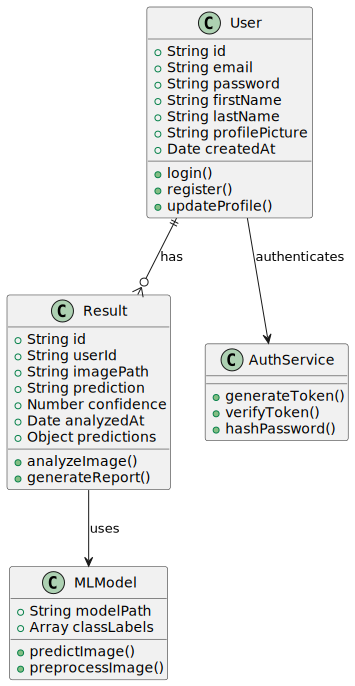
\includegraphics[width=0.4\linewidth]{Images/Highlevel/class.pdf}
                  \caption{Class Diagram}
                  \label{fig:ClassDiagram}
              \end{figure}
          \end{center}
          The class diagram presents the fundamental building blocks of the brain tumor detection system. The User class serves as the central entity representing application users, containing basic authentication and profile information along with methods for login, registration, and profile updates. The Result class captures the outcomes of brain tumor analyses, storing prediction results, confidence scores, and timestamps while providing methods for image analysis and report generation. The MLModel class abstracts the machine learning functionality, encapsulating the model path and class labels with methods for image prediction and preprocessing. The AuthService class handles security operations including token generation, verification, and password hashing. The relationships show that users can have multiple analysis results, results utilize the ML model for predictions, and users interact with the authentication service for security purposes.



    \item \textbf{Object Diagram}
          \begin{center}
              \begin{figure}[H]
                  \centering
                  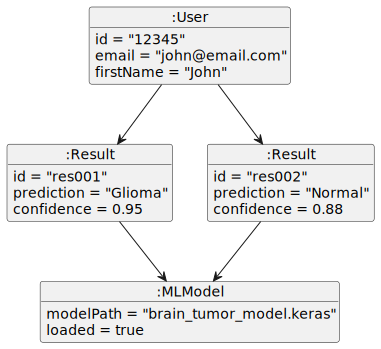
\includegraphics[width=0.60\linewidth]{Images/Highlevel/object.pdf}
                  \caption{Object Diagram}
                  \label{fig:ObjectDiagram}
              \end{figure}
          \end{center}
          This object diagram illustrates a specific runtime scenario where a user named John has performed brain tumor analyses. The diagram shows concrete instances of the classes, with User object ``12345'' representing John's account information, connected to two Result objects showing actual analysis outcomes -- one detecting a Glioma tumor with 95\% confidence and another showing a Normal scan with 88\% confidence. Both results are linked to the same MLModel instance that has successfully loaded the Keras model file. This snapshot demonstrates how the system maintains relationships between users and their analysis history while sharing the ML model instance across multiple predictions.

          \newpage
    \item \textbf{State Diagram}
          \begin{center}
              \begin{figure}[H]
                  \centering
                  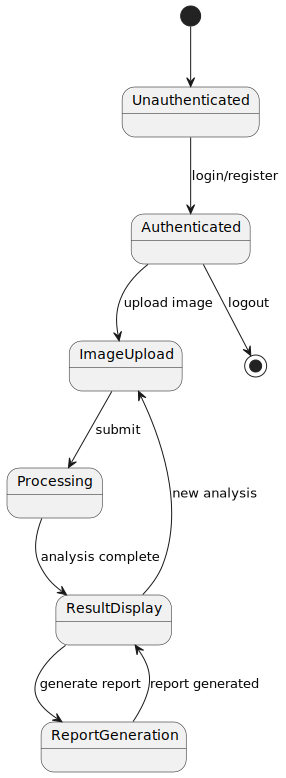
\includegraphics[width=0.35\linewidth]{Images/Highlevel/state.pdf}
                  \caption{State Diagram}
                  \label{fig:StateDiagram}
              \end{figure}
          \end{center}
          The state diagram traces the user journey through the application's main workflow states. Users begin in an unauthenticated state and transition to authenticated status through successful login or registration. Once authenticated, users can navigate to image upload functionality, where they submit brain scan images for analysis. The system then moves to a processing state where the ML model analyzes the uploaded image. Upon completion, users reach the result display state where they can view their analysis outcomes. From this state, users can either initiate new analyses by returning to image upload or generate detailed PDF reports. The diagram also shows the logout transition that returns users to the unauthenticated state, completing the application lifecycle. This workflow represents the essential data flow from image submission to result presentation.


    \item \textbf{Sequence Diagram}
          \begin{center}
              \begin{figure}[H]
                  \centering
                  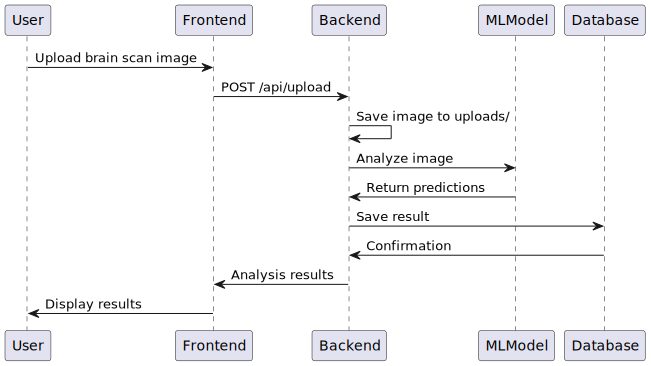
\includegraphics[width=0.9\linewidth]{Images/Highlevel/sequence.pdf}
                  \caption{Sequence Diagram}
                  \label{fig:SequenceDiagram}
              \end{figure}
          \end{center}
          This sequence diagram depicts the core interaction flow for brain tumor analysis. The process begins when a user uploads a brain scan image through the frontend interface. The frontend forwards this request to the backend server, which first saves the uploaded image to the designated uploads directory. The backend then invokes the ML model service to analyze the saved image, receiving prediction results including tumor classification and confidence scores. These results are subsequently stored in the database for future reference and user history. The backend returns the analysis results to the frontend, which presents them to the user in a comprehensible format. This workflow represents the essential data flow from image submission to result presentation.


    \item \textbf{Activity Diagram} \\
          The activity diagram outlines the decision-based workflow of the application. The process starts with authentication verification, directing unauthenticated users through the login process before proceeding. Once authenticated, users can upload images, which undergo validation to ensure they meet the system requirements for format and size. Valid images proceed to ML model processing, where the deep learning algorithm analyzes the brain scan for tumor detection. Successful analysis results are saved to the database and displayed to users. The workflow includes an optional branch for PDF report generation, allowing users to create downloadable documentation of their analysis results. Error handling is integrated throughout, redirecting users to appropriate error states when validation or processing fails.
          \begin{center}
              \begin{figure}[H]
                  \centering
                  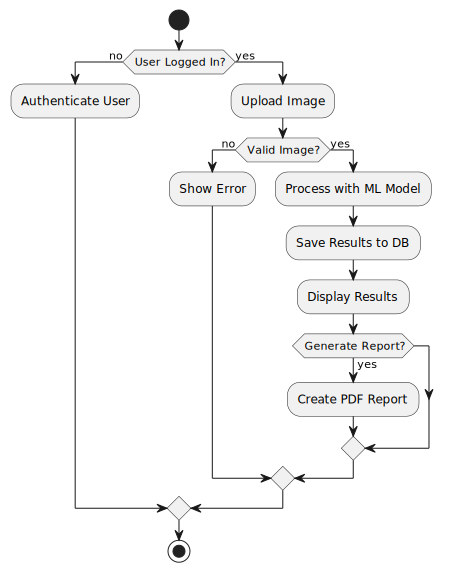
\includegraphics[width=0.70\linewidth]{Images/Highlevel/activity.pdf}
                  \caption{Activity Diagram}
                  \label{fig:ActivityDiagram}
              \end{figure}
          \end{center}
\end{enumerate}

\subsection{Activities Performed}

\newpage
\stepcounter{section}
\section*{\Large\centering {CHAPTER 4 \\ SYSTEM DESIGN}}
\addcontentsline{toc}{section}{CHAPTER 4: System Design}\label{4}
\subsection{Design}
System design takes the findings from analysis and converts them into a
practical plan for development. It describes the system’s architecture,
components, data flow, and deployment environment. The design ensures that each
part of the system frontend, backend, database, and machine learning model
works together smoothly. Diagrams like class, sequence, and deployment diagrams
help visualize the structure and workflow, making implementation easier and
more reliable.
\begin{enumerate}[label=\roman*.]
    \item \textbf{Class Diagram}
          \begin{center}
              \begin{figure}[H]
                  \centering
                  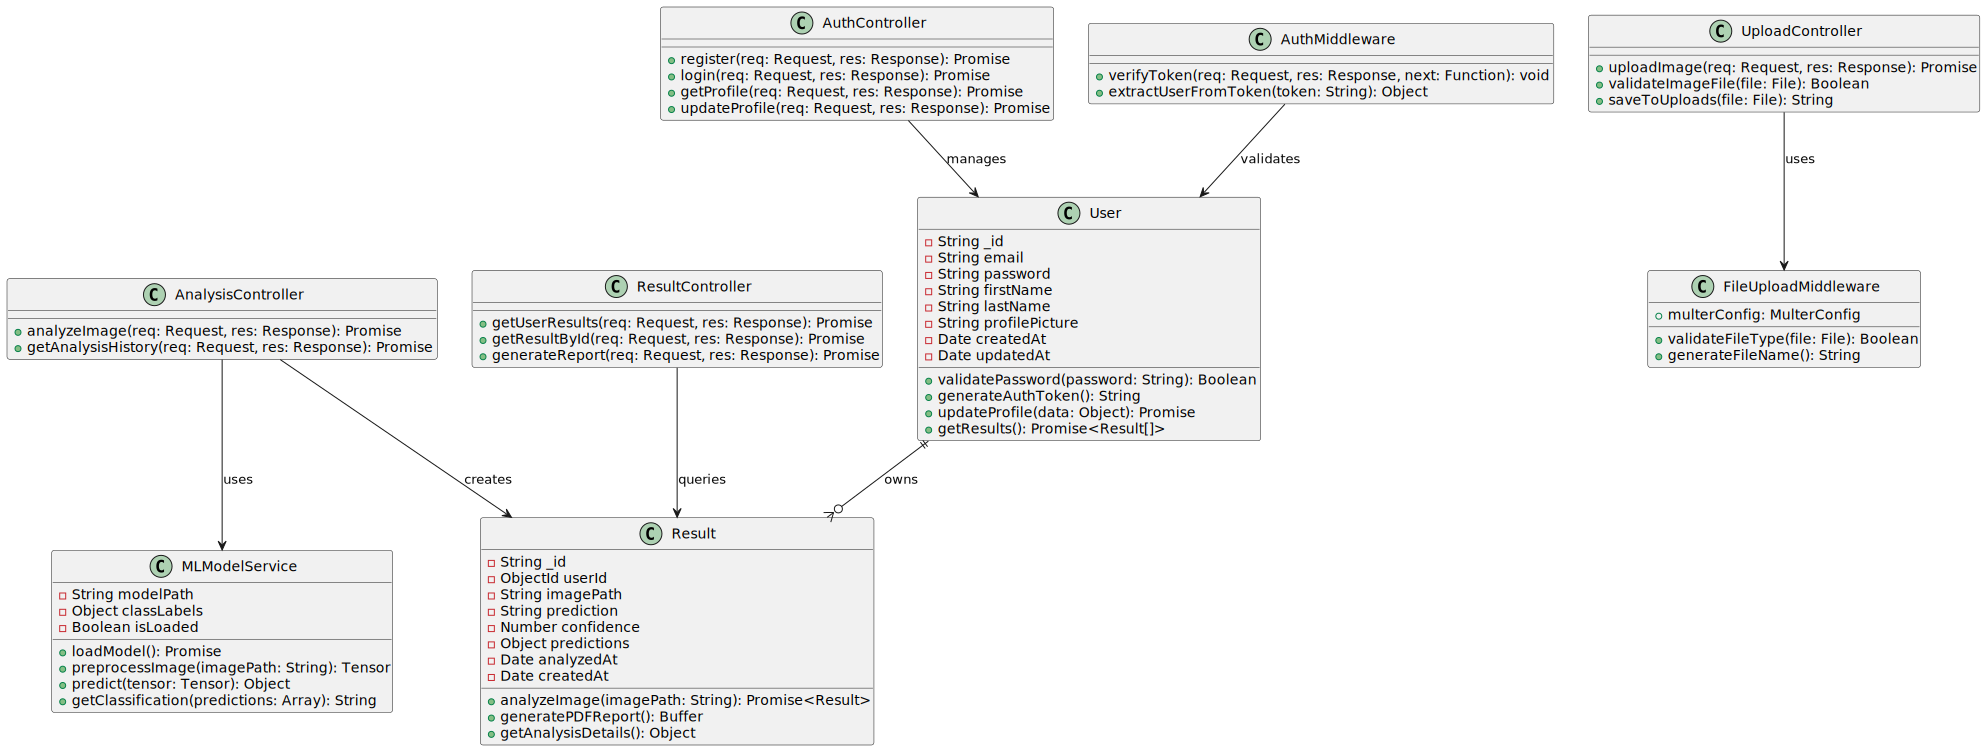
\includegraphics[width=1\linewidth]{Images/Refined/class.pdf}
                  \caption{Refinement of Class Diagram}
                  \label{fig:RefinementofClassDiagram}
              \end{figure}
          \end{center}
          The refined class diagram significantly expands upon the high-level version by introducing detailed implementation specifics and architectural components. While the original diagram focused on core domain entities, this version incorporates the complete MVC architecture with dedicated controller classes for different functional areas. The AuthController, UploadController, AnalysisController, and ResultController represent the application's API endpoints and business logic handlers. New middleware components like AuthMiddleware and FileUploadMiddleware demonstrate the request processing pipeline and security layers. The MLModelService class provides more granular methods for model loading, image preprocessing, tensor operations, and classification logic. Database models now include private fields with proper encapsulation and detailed method signatures showing parameter types and return values. This refined diagram reveals the actual software architecture with separation of concerns, dependency injection patterns, and proper abstraction layers that weren't visible in the high-level overview.
    \item \textbf{Object Diagram}
          \begin{center}
              \begin{figure}[H]
                  \centering
                  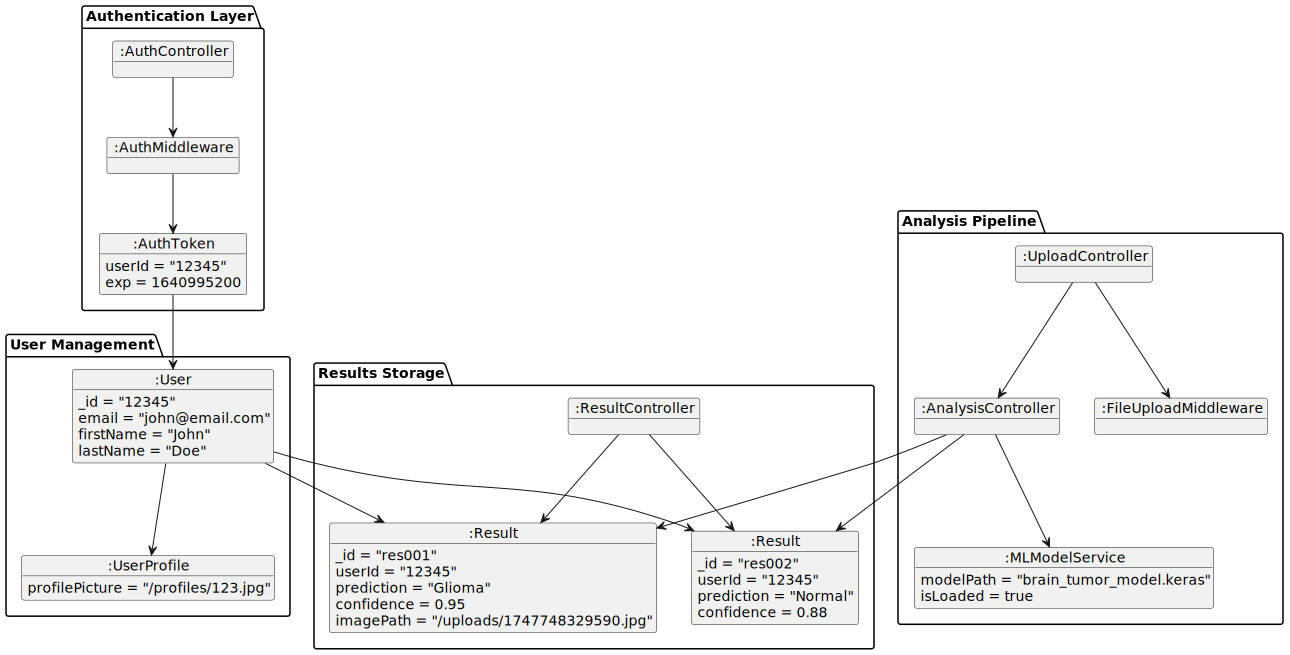
\includegraphics[width=1\linewidth]{Images/Refined/obj.pdf}
                  \caption{Refinement of Object Diagram}
                  \label{fig:RefinementofObjectDiagram}
              \end{figure}
          \end{center}
          The refined object diagram presents a more comprehensive runtime view by organizing components into logical packages representing different architectural layers. Unlike the simple high-level version, this diagram shows the Authentication Layer with controller instances, middleware objects, and JWT token representations. The User Management package demonstrates the relationship between user entities and their profile information. The Analysis Pipeline package reveals the complete request processing flow from upload controllers through file middleware to ML services. The Results Storage package shows how multiple result instances are managed by dedicated controllers. This detailed view exposes the actual object collaboration patterns, package dependencies, and layer interactions that occur during system execution, providing insights into the implementation architecture that the high-level diagram abstracted away.

    \item \textbf{State Diagram} \\
          The refined state diagram transforms the simple linear workflow into a comprehensive state machine with nested states and complex transitions. The original diagram showed basic authentication and analysis states, while this version introduces hierarchical state organization with distinct flows for authentication, image analysis, and profile management. The AuthenticationFlow composite state includes detailed substates for token checking, form validation, and error handling.
          \begin{center}
              \begin{figure}[H]
                  \centering
                  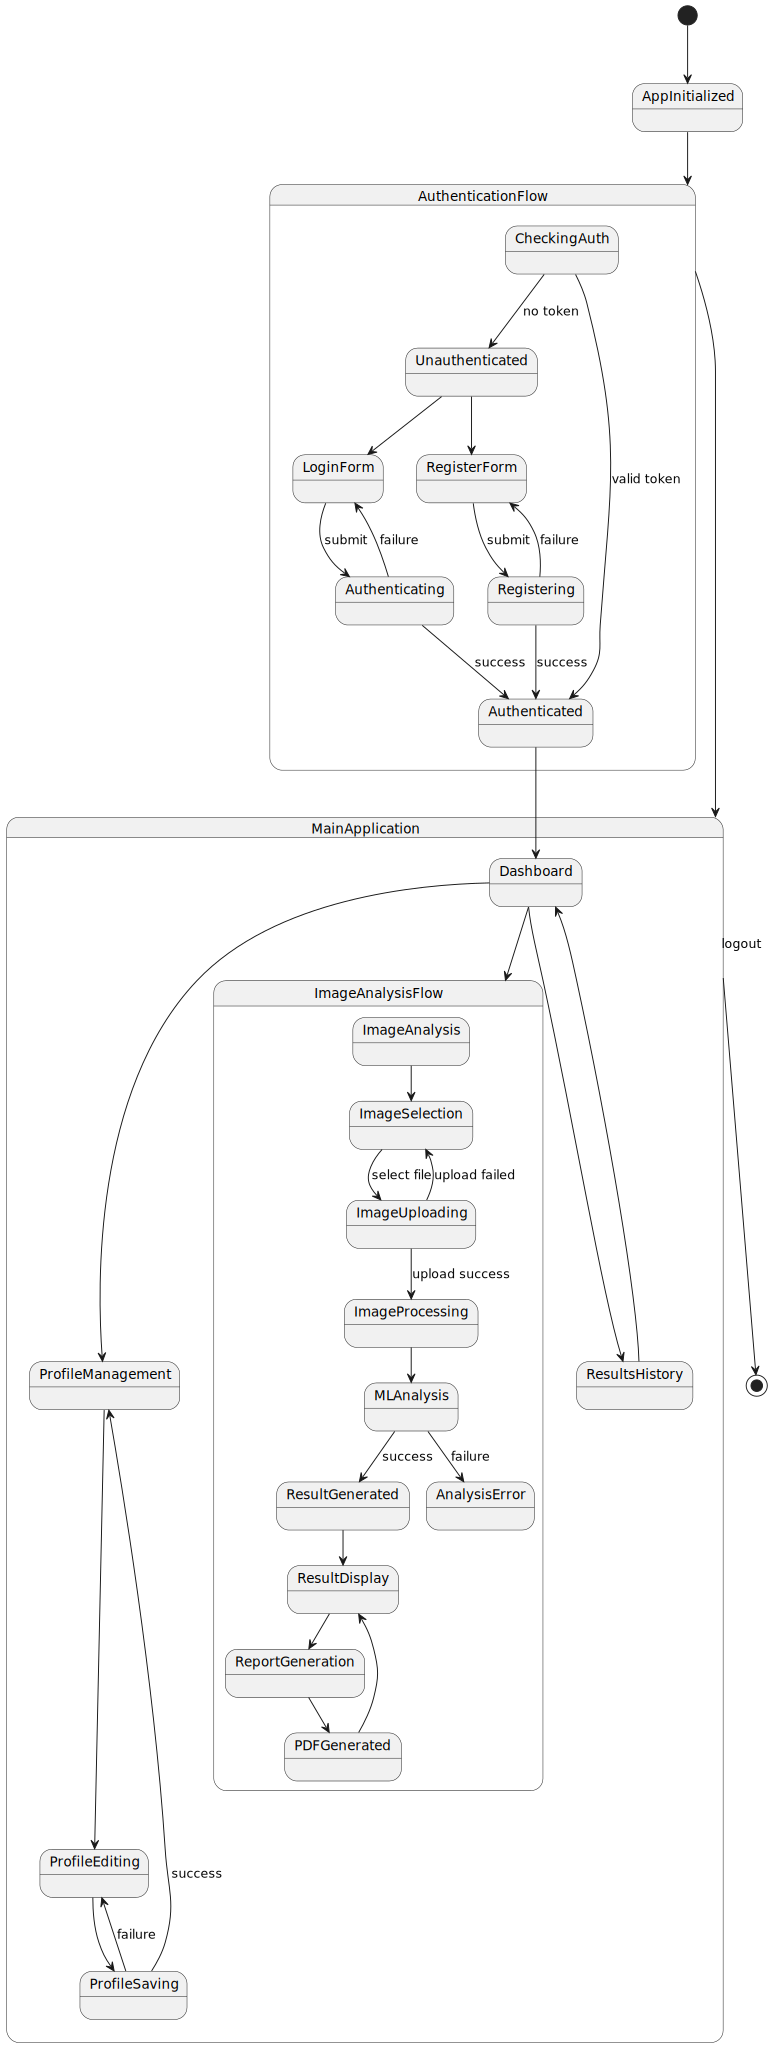
\includegraphics[width=0.6\linewidth]{Images/Refined/state.pdf}
                  \caption{Refinement of State Diagram}
                  \label{fig:RefinementofStateDiagram}
              \end{figure}
          \end{center}
          The ImageAnalysisFlow demonstrates the complete image processing pipeline with states for selection, uploading, processing, ML analysis, result generation, and error recovery. Additional states for profile management and report generation show parallel user workflows. This refined diagram captures real-world application complexity with multiple concurrent processes, error states, and recovery mechanisms that provide a complete picture of system behavior under various conditions.
    \item \textbf{Sequence Diagram}
          \begin{center}
              \begin{figure}[H]
                  \centering
                  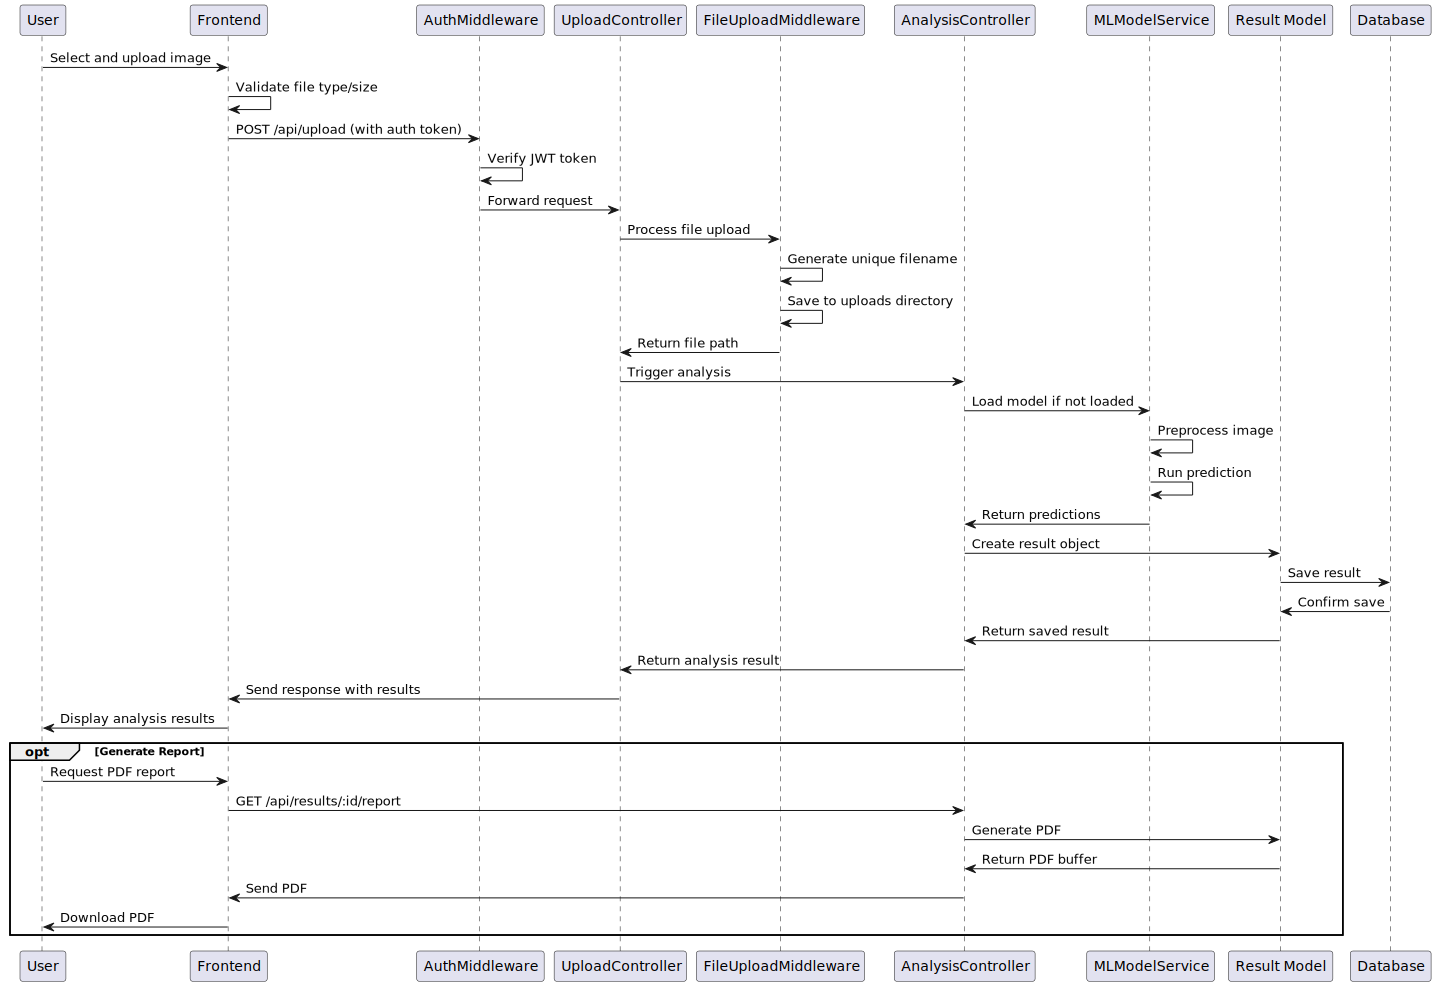
\includegraphics[width=1\linewidth]{Images/Refined/sequence.pdf}
                  \caption{Refinement of Sequence Diagram}
                  \label{fig:RefinementofSequenceDiagram}
              \end{figure}
          \end{center}
          The refined sequence diagram expands the simple high-level interaction into a detailed multi-participant collaboration showing the complete request processing pipeline. While the original diagram showed basic frontend-backend-model communication, this version reveals the actual middleware stack, authentication verification, file processing layers, and database operations. The diagram now includes AuthMiddleware for token verification, FileUploadMiddleware for file handling, and separate controllers for different responsibilities. Additional detail shows model loading optimization, image preprocessing steps, database confirmation patterns, and optional PDF generation workflows. Error handling scenarios and alternative flows are represented through optional fragments. This comprehensive view demonstrates the actual software architecture with proper separation of concerns, middleware processing, and the complete data transformation pipeline from user input to final output.

    \item \textbf{Activity Diagram}
          \begin{center}
              \begin{figure}[H]
                  \centering
                  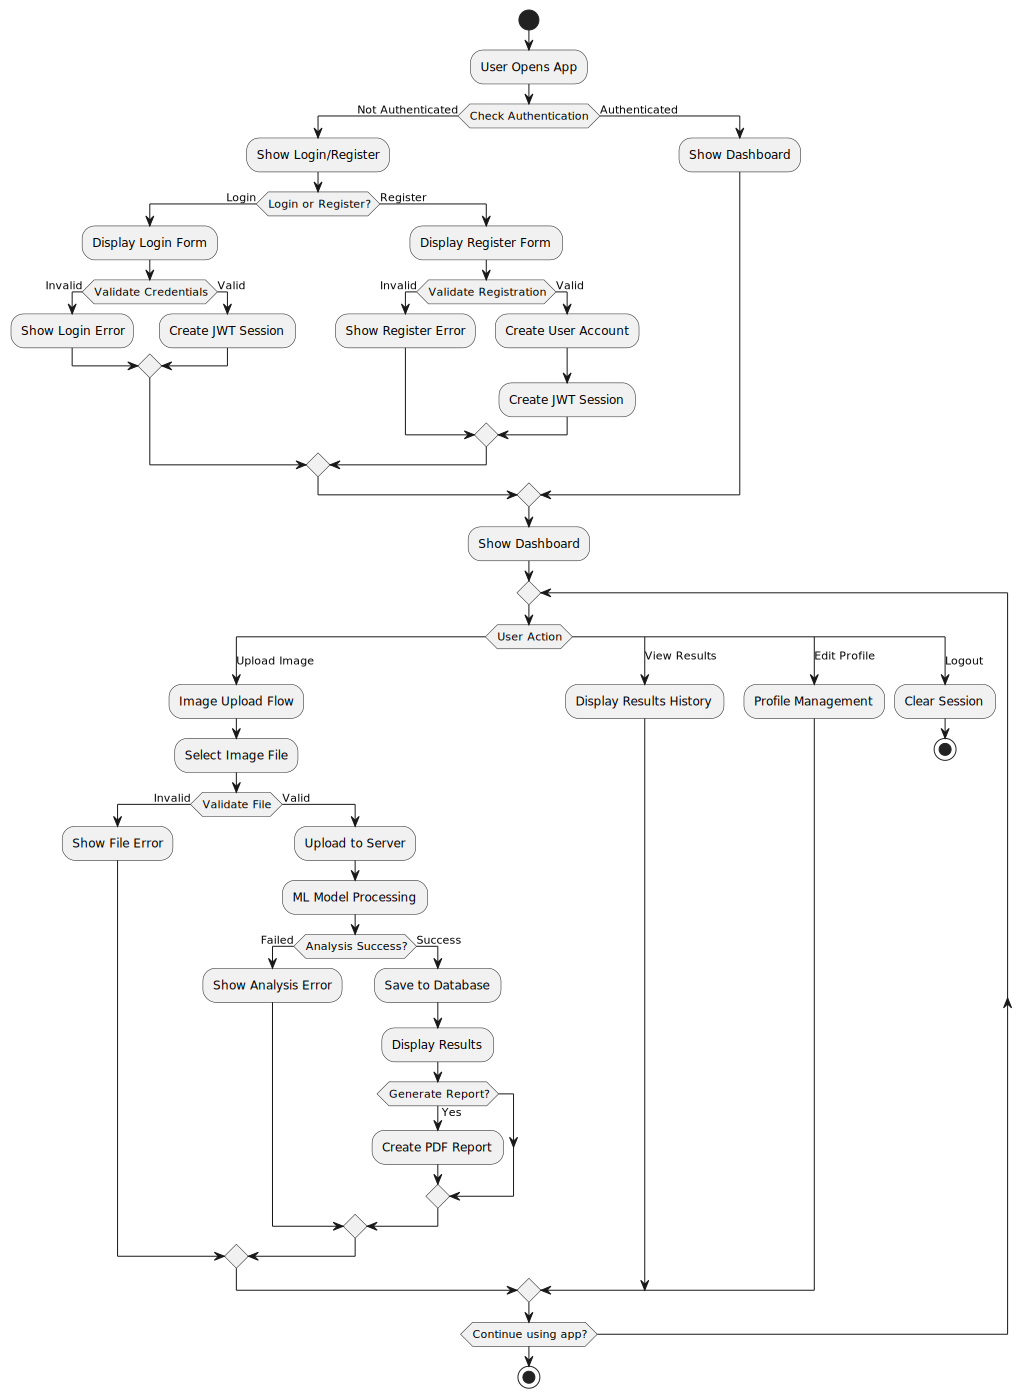
\includegraphics[width=0.8\linewidth]{Images/Refined/activity.pdf}
                  \caption{Refinement of Activity Diagram}
                  \label{fig:RefinementofActivityDiagram}
              \end{figure}
          \end{center}
          The refined activity diagram transforms the basic decision flow into a comprehensive business process model with detailed error handling and multiple workflow branches. The high-level diagram showed simple authentication and analysis paths, while this version incorporates complete user registration flows, detailed validation processes, and comprehensive error recovery mechanisms. New branches handle user account creation, profile management workflows, and multiple analysis result viewing options. The diagram now shows parallel processes for different user actions, detailed file validation steps, and granular ML processing phases. Error states are properly connected to recovery paths, and the workflow includes session management, logout procedures, and application lifecycle management. This detailed process model reflects the actual user experience with all possible paths, decision points, and system responses that users encounter during real application usage.
    \item \textbf{Component Diagram}
          \begin{center}
              \begin{figure}[H]
                  \centering
                  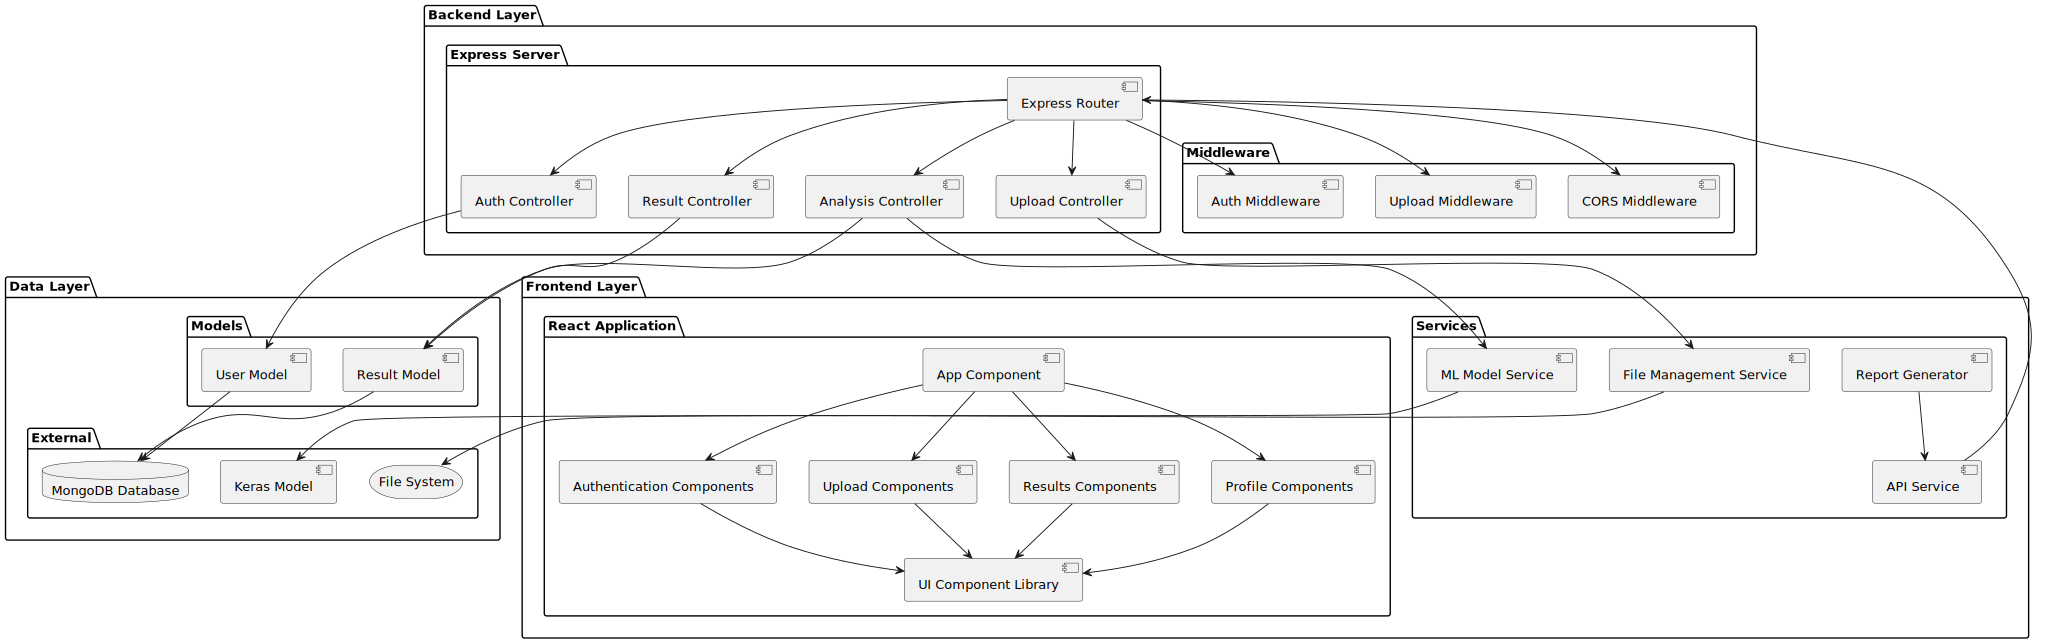
\includegraphics[width=1\linewidth]{Images/Refined/component.pdf}
                  \caption{Refinement of Component Diagram}
                  \label{fig:RefinementofComponentDiagram}
              \end{figure}
          \end{center}
          The component diagram presents the system's architectural organization across three distinct layers, demonstrating how components collaborate to deliver application functionality. The Frontend Layer contains the React application with its constituent components for authentication, file upload, results display, and profile management, all built upon a shared UI component library. The API Service and Report Generator provide client-side services for server communication and document generation. The Backend Layer implements the Express server architecture with route handlers, controllers for different functional domains, and middleware components for cross-cutting concerns like authentication, file upload processing, and CORS handling. Business logic services handle ML model operations and file management. The Data Layer abstracts database operations through Mongoose models while connecting to external systems including MongoDB for data persistence, the file system for image storage, and the Keras model for machine learning predictions. This organization demonstrates clear separation of concerns with defined interfaces between layers.
          \newpage
    \item \textbf{Deployment Diagram}
          \begin{center}
              \begin{figure}[H]
                  \centering
                  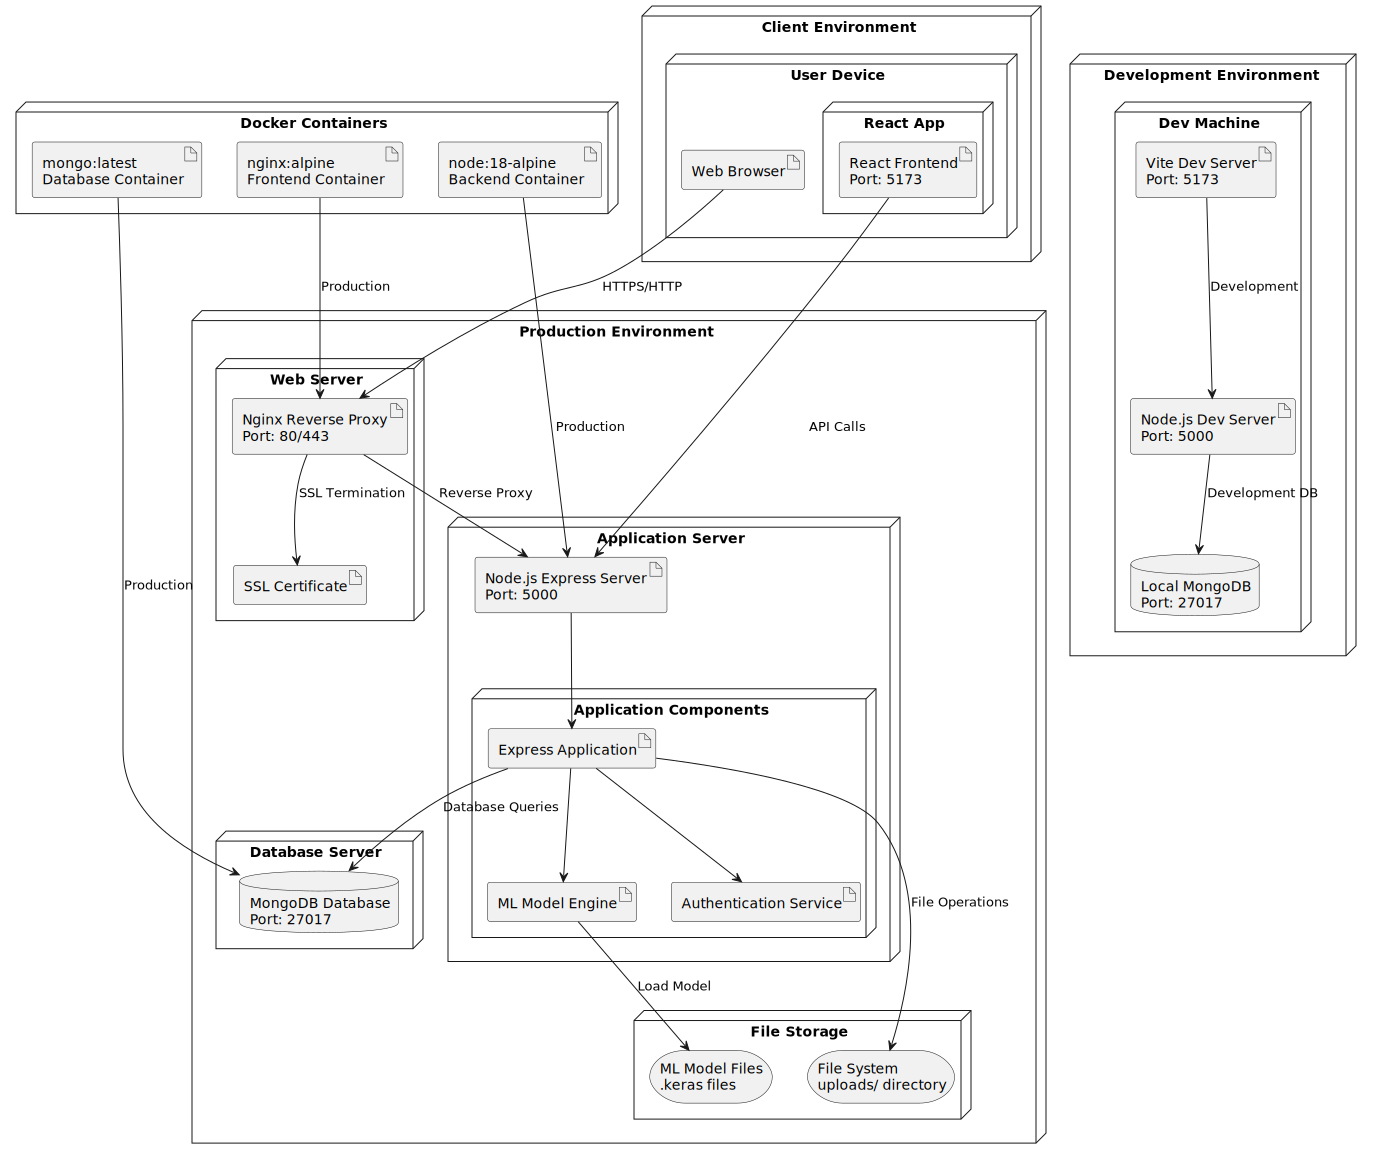
\includegraphics[width=1\linewidth]{Images/Refined/deployment.pdf}
                  \caption{Refinement of Deployment Diagram}
                  \label{fig:RefinementofDeploymentDiagram}
              \end{figure}
          \end{center}
          The deployment diagram illustrates the complete system infrastructure across development, production, and containerized environments. The Client Environment shows end-user devices running web browsers that host the React frontend application. The Production Environment demonstrates a multi-tier architecture with Nginx serving as a reverse proxy and SSL termination point, forwarding requests to the Node.js application server. The application server hosts the Express framework with integrated ML model engine and authentication services, connecting to a dedicated MongoDB database server and file storage systems for uploads and model files. The Development Environment mirrors production with local development servers and database instances for testing. Docker containerization provides deployment flexibility with separate containers for frontend, backend, and database components. This infrastructure supports scalability, security, and maintainability while providing development-production parity through containerized deployments that ensure consistent environments across different deployment targets.
\end{enumerate}

\subsection{Algorithm Details}
\textbf{Convolutional Neural Network (\gls{cnn})}

A \gls{cnn} is a type of artificial neural network specifically designed for
processing and classifying visual data. In this project, we developed a custom
\gls{cnn} architecture tailored for medical imaging.

The primary algorithm powering the brain tumor detection system is a
Convolutional Neural Network implemented using TensorFlow/Keras framework. This
deep learning algorithm employs multiple convolutional layers with ReLU
activation functions, pooling layers for dimensionality reduction, and fully
connected dense layers for final classification~\cite{krizhevsky2012imagenet}.
The CNN automatically learns hierarchical features from brain MRI images,
starting with simple edge detection in early layers and progressing to complex
anatomical structures in deeper layers. The network architecture includes batch
normalization for training stability~\cite{ioffe2015batch}, dropout layers for
regularization to prevent overfitting~\cite{srivastava2014dropout}, and a
softmax output layer that produces probability distributions across four
classes: Glioma, Meningioma, Pituitary tumors, and Normal brain scans. The
algorithm processes 224$ \times$ 224 pixel RGB images and outputs confidence
scores for each tumor category, enabling medical professionals to assess the
reliability of predictions alongside the primary classification result.

\begin{figure}[H]
    \centering
    \includegraphics[width=0.85\linewidth]{Images/cnn.png}
    \caption{CNN Architecture}
    \label{fig:CNN Architecture}
\end{figure}

\textbf{Transfer Learning with \gls{vgg16}}

To complement the custom \gls{cnn} and further enhance accuracy, we integrate a
transfer learning approach using the \gls{vgg16} architecture pretrained on the
ImageNet dataset. \gls{vgg16} is a well-established deep network known for its
simplicity and performance in image classification tasks.

In our approach, the \gls{vgg16} base model is used without its top
classification layers. All convolutional layers of \gls{vgg16} are frozen to
retain the pretrained features, which are known to capture generic visual
patterns that are also relevant to medical images.

On top of the \gls{vgg16} base, we add a Global Average Pooling layer followed
by fully connected Dense layers with \gls{relu} activations and Dropout. The
final classification layer uses softmax activation to output probabilities for
each class. This hybrid model combines the general visual understanding of
\gls{vgg16} with task-specific learning layers adapted to brain tumor
detection.

\begin{figure}[H]
    \centering
    \includegraphics[width=0.85\linewidth]{Images/vgg16.jpg}
    \caption{VGG16 Architecture}
    \label{fig:VGG16 Architecture}
\end{figure}

\textbf{JSON Web Token (JWT) Authentication Algorithm}

The stateless authentication mechanism employs JSON Web Tokens to manage user
sessions and API access control~\cite{jwtio_introduction}. The JWT algorithm
creates digitally signed tokens containing user identity information and access
permissions, typically using Hash-based Message Authentication Code with
\gls{sha256} or \gls{rsa} algorithms for signature
generation~\cite{jwtio_introduction}. Upon successful login, the server
generates a JWT containing the user's ID, email, role, and expiration
timestamp, signing it with a secret key to ensure its integrity and
authenticity. The algorithm enables distributed authentication without
requiring server-side session storage, as each token carries sufficient
information for access verification. Token validation involves signature
verification using the same secret key, expiration time checking, and payload
extraction for user identification. The implementation includes automatic token
refresh mechanisms and secure transmission protocols to maintain session
security while providing seamless user experience across multiple application
components.

\textbf{Bcrypt Password Hashing Algorithm}

The authentication security relies on the bcrypt algorithm for secure password
storage and verification~\cite{geeksforgeeks_bcrypt}. This adaptive hashing
function incorporates a configurable salt parameter that increases
computational complexity and prevents rainbow table attacks. The algorithm
generates unique salt values for each password, combines them with the
plaintext password, and applies multiple rounds of hashing using the Blowfish
cipher~\cite{geeksforgeeks_bcrypt}. The system implements a minimum of 12 salt
rounds, creating a computationally expensive operation that significantly slows
down brute-force attacks while remaining efficient for legitimate
authentication requests. The bcrypt algorithm automatically handles salt
generation and storage within the hash output, enabling seamless password
verification during user login attempts while maintaining resistance against
timing attacks and providing forward security as computational power increases
over time.



\newpage
\stepcounter{section}
\section*{\Large\centering {CHAPTER 5 \\ IMPLEMENTATION AND TESTING}}
\addcontentsline{toc}{section}{CHAPTER 5: Implementation and Testing}\label{5}
\subsection{Implementation}
\subsubsection{Tools Used}

\begin{enumerate}[label=\roman*.]
    \item \textbf{Frontend Development Tools:}
          \begin{enumerate}[label=$\bullet$]
              \item React.js \-- Primary frontend framework for building user interfaces
              \item TypeScript \-- Type-safe JavaScript for enhanced development experience
              \item Vite \-- Modern build tool and development server for fast compilation
              \item React Router \-- Declarative routing for React.js
              \item Shadcn/ui \-- UI component library built on Radix UI
              \item Lucide React \-- Open-source icon library
              \item Tailwind CSS \-- Utility-first CSS framework
          \end{enumerate}

    \item \textbf{State Management \& Hooks}
          \begin{enumerate}[label=$\bullet$]
              \item React Context API \-- Global state management for authentication
              \item React Hook Form \-- Form handling and validation library
          \end{enumerate}

    \item \textbf{Backend Development Tools}
          \begin{enumerate}[label=$\bullet$]
              \item Node.js \-- JavaScript runtime for server-side development
              \item Express.js \-- Web framework for Node.js
              \item JavaScript \-- Programming language for backend logic
              \item MongoDB \-- NoSQL database for data storage
          \end{enumerate}

    \item \textbf{Authentication \& Security}
          \begin{enumerate}[label=$\bullet$]
              \item Bcryptjs \-- Password hashing library
              \item Jsonwebtoken (JWT) \-- Token-based authentication
              \item Cors \-- Cross-Origin Resource Sharing middleware
          \end{enumerate}

    \item \textbf{File Handling}
          \begin{enumerate}[label=$\bullet$]
              \item Multer \-- Middleware for handling file uploads
          \end{enumerate}

    \item \textbf{Machine Learning \& AI Tools}
          \begin{enumerate}[label=$\bullet$]
              \item Tensorflow.js \-- Machine learning library for JavaScript
              \item Keras \-- High-level neural networks API
              \item Python \-- Primary language for ML implementation
          \end{enumerate}

    \item \textbf{Image Processing Tools}
          \begin{enumerate}[label=$\bullet$]
              \item OpenCV \-- Computer vision library
              \item PIL (Python Imaging Library) \-- Image manipulation library
              \item NumPy \-- Numerical computing library for array operations
          \end{enumerate}

    \item \textbf{Image Visualization Tools}
          \begin{enumerate}[label=$\bullet$]
              \item Matplotlib \-- Plotting and visualization library for Python
              \item Seaborn \-- Statistical data visualization library
              \item Sklearn \-- For Generating Model Evaluation Matrices
          \end{enumerate}

    \item \textbf{Model Components}
          \begin{enumerate}[label=$\bullet$]
              \item CNN \-- Convolutional Neural Network for image classification
              \item VGG16 \-- Pre-trained model for feature extraction
          \end{enumerate}

    \item \textbf{Development Environment Tools}
          \begin{enumerate}[label=$\bullet$]
              \item Visual Studio Code \-- Code editor with support for TypeScript, JavaScript and
                    Jupyter Notebooks
              \item Postman \-- API testing tool
              \item Docker \-- Containerization platform
              \item Git \-- Version control system
              \item Nginx \-- Web server and reverse proxy
          \end{enumerate}

\end{enumerate}

\subsubsection{Implementation Details of Modules}

\textbf{Dataset Overview}

This project utilizes publicly available \gls{mri} brain tumor datasets sourced
from the Kaggle machine learning platform Dataset available at:
\url{https://www.kaggle.com/datasets/masoudnickparvar/brain-tumor-mri-dataset}.
The comprehensive and well-curated dataset contains exactly 7,023 high-quality
\gls{mri} images that have been systematically categorized into four distinct
classes: glioma tumors, meningioma tumors, pituitary tumors, and cases with no
tumor present. All images are provided in standard grayscale JPG format with
varying dimensions, typically ranging from $240 \times 240$ to $512 \times 512$
pixels. Each image has been meticulously labeled according to its corresponding
tumor classification, making this dataset highly suitable for supervised
learning approaches and multi-class classification tasks. The dataset exhibits
minor class imbalance characteristics, necessitating careful attention and
specialized handling during preprocessing and dataset balancing phases.

\textbf{Data Preprocessing and Feature Extraction}

\gls{mri} images frequently contain various forms of noise, inconsistent brightness levels, and irrelevant background structures such as skull regions, which can negatively impact model performance and classification accuracy. Therefore, comprehensive preprocessing represents an essential and critical step in the methodology. The following systematic transformations are applied to enhance data quality:

\begin{enumerate}[label=\roman*.]
    \item Data augmentation techniques including random rotations, zooming operations,
          horizontal and vertical flipping, and spatial shifting are applied to
          artificially expand the dataset size and improve model generalization
          capabilities.
    \item Grayscale normalization and conversion to standardized 3-channel format for
          compatibility with pre-trained model architectures.
    \item Noise elimination using advanced morphological operations, specifically
          optimized combinations of erosion and dilation techniques.
    \item Skull-stripping procedures (when not already applied in the original dataset)
          to effectively isolate brain tissue regions of interest.
    \item Systematic resizing of all images to consistent dimensions: specifically $224
              \times 224$ pixels for \gls{vgg16} compatibility and $240 \times 240$ pixels
          for custom \gls{cnn} architectures, to match input requirements.
\end{enumerate}

Regarding feature extraction methodologies, the \gls{vgg16} model, pre-trained
on the comprehensive ImageNet dataset, serves as an effective feature
extractor. The initial convolutional layers are retained to leverage learned
low-level features including edges, textures, and basic shapes. The final
classification layers are systematically replaced and fine-tuned specifically
on brain \gls{mri} data to optimize tumor detection performance.

\textbf{Data Visualization and Dataset Balancing}

To comprehensively understand dataset characteristics, extensive exploratory
data visualization was performed using various analytical techniques and
statistical methods. The distribution of images across different tumor classes
was systematically analyzed using bar charts, histograms, and advanced
statistical plots. Additionally, representative random samples of \gls{mri}
scans from each category were displayed to facilitate visual inspection and
enhance understanding of distinct characteristics present in each tumor class.

Data visualization played a crucial role in identifying potential class
imbalance issues within the dataset structure. The dataset, containing labeled
\gls{mri} images indicating tumor presence or absence, exhibited some skewed
class distributions. These could potentially introduce bias during the model
training process. To effectively mitigate this bias, the ImageDataGenerator
class was strategically utilized with balanced sampling techniques. This
approach was implemented by configuring \texttt{class\_mode='categorical'} and
\texttt{shuffle=True} parameters, ensuring that training batches maintained
representative distributions across all tumor classes.

\textbf{Data Splitting}

The dataset was systematically partitioned into distinct training and
validation subsets using TensorFlow's \texttt{ImageDataGenerator} with a
carefully chosen validation split ratio of 20\%. This partitioning strategy
ensures that model performance is properly evaluated on previously unseen data
throughout the training process, providing reliable performance metrics. The
training generator was specifically configured with real-time data augmentation
techniques, including random rotations, zooming operations, shearing
transformations, and flipping operations to prevent overfitting and improve
model generalization capabilities across diverse image variations.

\begin{itemize}
    \item \textbf{Training Set:} Comprises 80\% of the total data, with comprehensive augmentation and shuffling applied.
    \item \textbf{Validation Set:} Contains 20\% of the data, used for continuous monitoring of model performance during training.
\end{itemize}

\textbf{Model Testing and Evaluation}

Following the completion of training phases, both the custom \gls{cnn}
architecture and the \gls{vgg16}-based transfer learning models were
comprehensively evaluated on a separate, independent test set to assess
real-world performance capabilities. Predictions were systematically generated
and results were compared against ground truth labels using multiple evaluation
metrics:

\begin{itemize}
    \item \textbf{Accuracy:} Calculated as the ratio of correctly predicted images to total test images.
    \item \textbf{Confusion Matrix:} Utilized for detailed analysis of true positives, false positives, true negatives, and false negatives across all classes.
    \item \textbf{Classification Report:} Provides comprehensive precision, recall, and F1-score metrics for each individual class.
\end{itemize}

These comprehensive metrics provided a holistic and detailed view of model
performance, revealing specific strengths and weaknesses in classifying tumor
versus non-tumor \gls{mri} scans. Advanced visualization of confusion matrices
and representative sample predictions facilitated interpretation of model
behavior and supported systematic refinement of the classification approach.


\subsection{Testing}
This project tests backend and frontend separately with tools suited to each
side. The backend uses \textbf{Jest} to run tests, Supertest to call the real
Express APIs, and an in-memory MongoDB so nothing touches your real database.
The frontend uses \textbf{Vitest} with \textbf{jsdom} to simulate a browser and
the \textbf{React Testing Library} to render components pages and simulate user
actions. The workflow is simple: write fast unit tests with mocks, then add
system tests to cover real flows. Heavy parts (like ML inference) are mocked so
runs are quick and reliable.

\subsubsection{Test Cases for Unit Testing}

For the frontend, the testing mainly focuses on checking small parts of the app
in a controlled, fake browser environment. Utility functions are verified by
making sure they return the right results, and the API service is tested with
fake HTTP requests so we can confirm things like requests, token handling, and
error cases without calling a real server. User interface pieces—such as
protected routes, the navbar with theme toggling, and the profile editor—are
tested using React Testing Library. Here, network calls are mocked and
real-world actions like typing, clicking, or uploading a file are simulated to
see if everything behaves as expected.

On the backend, testing is done by isolating middleware, models, and
controllers to make sure each works properly on its own. For example, the
authentication middleware is tested with different headers to ensure invalid
tokens are blocked while valid ones attach the user correctly. The user model
is checked using an in-memory database to confirm password hashing and
comparison work correctly. Controllers are tested with mocked setups: the
analysis controller fakes the Python process to test input and output handling,
while the upload controller checks for errors when files are missing and makes
sure temporary files are cleaned up. All external tasks like filesystem access
or subprocess calls are mocked to keep the tests fast and reliable.

\begin{table}[h!]
    \centering
    \caption{Summary of Unit Test Results}
    \begin{tabularx}{\textwidth}{lXl}
        \toprule
        \textbf{Test File}                            & \textbf{Test Description}                             & \textbf{Result / Time} \\
        \midrule
        \_\_tests\_\_/unit/authMiddleware.test.js     & rejects missing authorization header                  & PASS (3 ms)            \\
                                                      & rejects malformed authorization header                & PASS (1 ms)            \\
                                                      & accepts valid token and attaches userId               & PASS (7 ms)            \\
                                                      & rejects invalid token                                 & PASS (15 ms)           \\
        \midrule
        \_\_tests\_\_/unit/uploadController.test.js   & returns 400 when no file in uploadTempFile            & PASS (1 ms)            \\
                                                      & returns success when file provided                    & PASS                   \\
                                                      & cleanupTempFiles deletes older files beyond threshold & PASS (11 ms)           \\
        \midrule
        \_\_tests\_\_/unit/analysisController.test.js & returns 400 when no file                              & PASS (1 ms)            \\
                                                      & saves result and returns prediction on success        & PASS (8 ms)            \\
        \midrule
        \_\_tests\_\_/unit/userModel.test.js          & hashes password on save and compares correctly        & PASS (328 ms)          \\
        \bottomrule
    \end{tabularx}
\end{table}

\noindent\textbf{Test Suites:} 4 passed, 4 total \\
\textbf{Tests:} 10 passed, 10 total \\
\textbf{Snapshots:} 0 total \\
\textbf{Time:} 2.855 s \\
\textbf{Results written to:} test-results/unit.json

\subsubsection{Test Cases for System Testing}
For the frontend, system-level tests bring different parts of the app together
to mimic how a real user would interact with it, while still faking the
network. The tests start the app on protected routes to check that users who
aren’t logged in get redirected to the login page. Once valid credentials are
entered, they confirm that tokens are saved and navigation works as expected.
The analysis flow is tested by uploading an image and making sure the predicted
label and confidence show up, while the profile flow checks that existing user
data loads, fields can be updated, and avatar uploads work with proper
feedback. These tests essentially confirm that full pages behave correctly end
to end inside the browser, without needing a live backend.

\begin{table}[h!]
    \centering
    \caption{Summary of Frontend Test Results}

    \begin{tabularx}{\textwidth}{lXl}
        \toprule
        \textbf{Test File / Component}   & \textbf{Test Description}                                   & \textbf{Time} \\
        \midrule
        src/test/api.auth.test.ts        & 5 tests (all passed)                                        & 149 ms        \\
        src/test/reportGenerator.test.ts & 4 tests (all passed)                                        & 18 ms         \\
        src/test/UserProfile.test.tsx    & UserProfile loads and displays profile data from API        & -             \\
        \midrule
        src/test/NavbarTheme.test.tsx    & 2 tests (all passed)                                        & 841 ms        \\
        Navbar and ThemeProvider         & renders auth links and triggers logout                      & 729 ms        \\
        \midrule
        src/test/LoginPage.test.tsx      & 2 tests (all passed)                                        & 956 ms        \\
        Login page                       & shows error when fields empty                               & 552 ms        \\
        Login page                       & logs in successfully and stores token                       & 391 ms        \\
        \midrule
        src/test/ProtectedRoute.test.tsx & 3 tests (all passed)                                        & 105 ms        \\
        \midrule
        src/test/UserProfile.test.tsx    & 3 tests (all passed)                                        & 1674 ms       \\
        UserProfile                      & loads and displays profile data from API                    & 474 ms        \\
        UserProfile                      & edits and saves profile via updateProfile                   & 1022 ms       \\
        UserProfile                      & shows error message on API failure                          & 176 ms        \\
        \midrule
        src/test/AnalysisPage.test.tsx   & 2 tests (all passed)                                        & 1146 ms       \\
        Analysis page                    & runs analysis and displays result summary                   & 846 ms        \\
        \midrule
        src/test/AppRoutes.test.tsx      & 2 tests (all passed)                                        & 583 ms        \\
        App routes                       & redirects unauthenticated user to /login on protected route & 488 ms        \\
        \bottomrule
    \end{tabularx}


\end{table}

\noindent
\textbf{Test Files:} 8 passed (8) \\
\textbf{Tests:} 23 passed (23) \\
\textbf{Start Time:} 23:50:25 \\
\textbf{Duration:} 6.76 s (transform 2.95s, setup 4.69s, collect 12.24s, tests 5.47s, environment 11.23s, prepare 4.56s)

For the backend, system tests run against the actual Express app with a
separate test database to cover complete API workflows. The authentication
journey is tested from start to finish, including registering, logging in to
receive a JWT, and accessing protected endpoints, with extra checks for edge
cases like duplicate accounts or wrong passwords. The results flow verifies
that uploading an image stores the result, allows listing results, and
retrieves them by ID, while also making sure one user cannot access another
user’s data and that invalid IDs return proper errors. Profile-related tests
confirm that user details can be fetched and updated, avatars can be uploaded,
and old avatars are properly cleaned up when replaced. Together, these tests
provide confidence that routing, validation, data handling, and security are
all working as intended.

\begin{table}[h!]
    \centering
    \caption{Summary of Backend Test Results}

    \begin{tabularx}{\textwidth}{lXl}
        \toprule
        \textbf{Test File / Component}               & \textbf{Test Description}                                & \textbf{Time} \\
        \midrule
        \_\_tests\_\_/system/results.e2e.test.js     & analyze image and then list results and get by id        & 37 ms         \\
                                                     & results API requires auth                                & 2 ms          \\
        \midrule
        \_\_tests\_\_/system/profile.e2e.test.js     & GET /api/profile returns current profile                 & 9 ms          \\
                                                     & PUT /api/profile updates basic fields                    & 12 ms         \\
                                                     & POST /api/profile/avatar uploads avatar and replaces old & 19 ms         \\
        \midrule
        \_\_tests\_\_/system/results-acl.e2e.test.js & User B cannot access User A result (403)                 & 12 ms         \\
                                                     & Requesting nonexistent result returns 404                & 9 ms          \\
        \midrule
        \_\_tests\_\_/system/auth.e2e.test.js        & register → login → get current user                      & 212 ms        \\
                                                     & login fails with wrong password                          & 154 ms        \\
                                                     & duplicate registration is rejected                       & 89 ms         \\
        \bottomrule
    \end{tabularx}

\end{table}

\noindent
\textbf{Test Suites:} 4 passed, 4 total \\
\textbf{Tests:} 10 passed, 10 total \\
\textbf{Snapshots:} 0 total \\
\textbf{Time:} 5.406 s \\
\textbf{Results written to:} test-results/system.json

\subsection{Result Analysis}

% The training process was effective, as shown by the consistent increase in
% accuracy and decrease in loss over 14 epochs. This indicates the model learned
% well and is not overfitting, with a strong overall accuracy of 97.25\%.

% The model is highly successful at differentiating tumor types. The ROC curves
% show a perfect AUC of 1.00 for every class, demonstrating its superior ability
% to distinguish between meningioma, glioma, pituitary, and non-tumor cases. This
% is supported by high precision, recall, and F1-scores for each class, all above
% 0.95.

% The confusion matrix confirms the model's low error rate. The number of correct
% predictions is significantly higher than misclassifications, showing the
% model's strong ability to accurately identify each specific class.

\begin{table}[h!]
\centering
\caption{Classification Report}
\begin{tabular}{lcccc}
\hline
\textbf{Class} & \textbf{Precision} & \textbf{Recall} & \textbf{F1-score} & \textbf{Support} \\
\hline
Meningioma & 0.93 & 0.97 & 0.95 & 306 \\
Glioma     & 0.98 & 0.94 & 0.96 & 300 \\
Notumor    & 0.99 & 0.99 & 0.99 & 405 \\
Pituitary  & 0.98 & 0.98 & 0.98 & 300 \\
\hline
\textbf{Accuracy} & \multicolumn{3}{c}{0.97} & 1311 \\
\textbf{Macro Avg} & 0.97 & 0.97 & 0.97 & 1311 \\
\textbf{Weighted Avg} & 0.97 & 0.97 & 0.97 & 1311 \\
\hline
\end{tabular}
\end{table}

\begin{table}[h!]
\centering
\caption{Overall Metrics}
\begin{tabular}{lc}
\hline
\textbf{Metric} & \textbf{Value} \\
\hline
Accuracy & 0.9725 \\
Precision (weighted) & 0.9729 \\
Recall (weighted) & 0.9725 \\
F1 Score (weighted) & 0.9726 \\
\hline
\end{tabular}
\end{table}


\begin{enumerate}[label=\roman*.]

\item \textbf{Receiver Operating Characteristic (ROC) Curve}

\begin{figure}[H]
    \centering
    \includegraphics[width=0.9\linewidth]{Images/Metrices/roc.png}
    \caption{ROC Curve for Brain Tumor Classification Model}
    \label{fig:VGG16 ROC Curve}
\end{figure}

Our model achieved an AUC of 1.0 for all individual classes (meningioma,
glioma, notumor, pituitary) and for the micro-average. This indicates that the
model is able to distinguish between the different classes with almost perfect
accuracy based on this metric. The curves are all hugging the top-left corner
of the graph, which is the optimal position. The dashed black line represents a
random classifier (AUC = 0.5).

\item \textbf{Precision, Recall, and F1-score}
\begin{figure}[H]
    \centering
    \includegraphics[width=1\linewidth]{Images/Metrices/scores.png}
    \caption{F1 Score, Precision, and Recall for VGG16 Model}
    \label{fig:VGG16 Scores}
\end{figure}

\begin{enumerate}
    \item \textbf{Precision}: Our model has high precision for all classes (above 0.95 for most), with "notumor" and "pituitary" being particularly high, indicating very few false positives.
    \item \textbf{Recall}: Our model also shows high recall across all classes, particularly for "notumor" and "pituitary," indicating it correctly identifies almost all instances of these classes.
    \item \textbf{F1-score}: The F1-scores are also very high (close to 0.98 for all classes), confirming the model's balanced performance in identifying classes correctly and comprehensively.
\end{enumerate}

\item \textbf{Model Training History}

\begin{figure}[H]
    \centering
    \includegraphics[width=1\linewidth]{Images/Metrices/traininghistory.png}
    \caption{Model Training History}
    \label{fig:Model Training History}
\end{figure}

This image shows the model's performance during the training process over 14 epochs.

\textbf{Model Accuracy:} The left plot shows both training accuracy (blue line) and validation accuracy (orange line). 
\begin{enumerate}[label=$\bullet$] 
    \item The training accuracy steadily increases and reaches a high of about 99\% by the final epoch.
    \item The validation accuracy also increases and closely follows the training accuracy, reaching a high of over 96\%.
    \item The closeness between the training and validation accuracy curves indicates that the model is learning effectively and generalizing well to new, unseen data, with no significant signs of overfitting.
\end{enumerate}

\textbf{Model Loss:} The right plot shows the training loss and validation loss.  
\begin{enumerate}[label=$\bullet$] 
    \item The training loss (blue line) decreases consistently throughout training, indicating the model is getting better at making correct predictions.
    \item The validation loss (orange line) also decreases, mirroring the training loss trend, which again suggests the model isn't overfitting. The validation loss shows some minor fluctuations, but the overall trend is a consistent decline.
\end{enumerate}

\item \textbf{Confusion Matrix}

\begin{figure}[H]
    \centering
    \includegraphics[width=1\linewidth]{Images/Metrices/confusion.png}
    \caption{Confusion Matrix for VGG16 Model}
    \label{fig:Confusion Matrix}
\end{figure}

The two heatmaps show the same data: the left one shows raw counts, and the right one shows normalized percentages.
\begin{enumerate}[label=$\bullet$] 

\item \textbf{Rows:} Represent the true labels (the actual class of the MRI).  

\item \textbf{Columns:} Represent the predicted labels (the class the model assigned).

\item \textbf{Diagonal Elements:} The numbers along the main diagonal (e.g., 293 for meningioma, 277 for glioma) represent the number of correct predictions for each class.

\item \textbf{Off-Diagonal Elements:} The numbers off the diagonal represent misclassifications.
\end{enumerate}

\textbf{Count Matrix (Left):} 
\begin{table}[h!]
\centering
\caption{Confusion matrix showing counts of correctly classified and misclassified MRI samples.}

\begin{tabular}{ccccc}
\toprule
\textbf{True Class} & \textbf{Meningioma} & \textbf{Glioma} & \textbf{Notumor} & \textbf{Pituitary} \\
\midrule
Meningioma & 293 & 3 & 2 & 8 \\
Glioma     & 18  & 277 & 0 & 5 \\
Notumor    & 0   & 0 & 401 & 0 \\
Pituitary  & 0   & 1 & 0 & 299 \\
\bottomrule
\end{tabular}
\end{table} 
% \begin{enumerate}[label=$\bullet$]
%     \item \textbf{Meningioma:} 293 were correctly classified, but 3 were mistaken for glioma, 2 for notumor, and 8 for pituitary.
%     \item \textbf{Glioma:} 277 were correct, but 18 were mistaken for meningioma, and 5 for pituitary.
%     \item \textbf{Notumor:} 401 were correct, with only a few misclassified.
%     \item \textbf{Pituitary:} 299 were correct, with only 1 misclassified as glioma.
% \end{enumerate}

\item \textbf{Normalized Matrix (Right):}  
\begin{enumerate}[label=$\bullet$]

\item This heatmap shows the same data as percentages of the total for each true class. 

\item The highest misclassification rate appears to be glioma being misclassified as meningioma (6\%), and meningioma being misclassified as pituitary (3\%). These are minor errors given the overall high accuracy.
\end{enumerate}
\end{enumerate}






\newpage
\stepcounter{section}
\section*{\Large\centering {CHAPTER 6 \\ CONCLUSION AND FUTURE RECOMMENDATIONS}}
\addcontentsline{toc}{section}{Conclusion and Future Recommendations}

\subsection{Conclusion}
The application provides an effective tool for analyzing brain MRI images and managing results. Users can upload images, receive predictions on tumor presence, and access past results along with profile management features. The frontend is built with React (Vite + Tailwind) served by Nginx, the backend uses Node/Express with MongoDB, and the ML model runs in Python. The system is thoroughly tested to ensure reliability and smooth deployment. The model demonstrates excellent performance, with almost all metrics above 0.97. Precision measures how many predicted positive cases were correct, recall measures how many actual positives were correctly identified, and F1-score balances precision and recall. Accuracy reflects overall correctness, support indicates sample counts per class, macro average treats all classes equally, and weighted average accounts for class size. Overall, the system achieves highly accurate tumor classification, making it a dependable tool for MRI analysis.
\subsection{Future Recommendations}
\begin{itemize}
    \item \textbf{Expand Model Types:} Include additional brain tumor types or other neurological conditions to improve coverage.
    \item \textbf{Improve User Interface:} Enhance UI/UX for easier navigation, visualization of results, and accessibility.
    \item \textbf{Strengthen Security:} Implement advanced authentication, encryption, and secure data storage practices.
    \item \textbf{Automate CI/CD:} Set up continuous integration and deployment pipelines for faster updates and maintenance.
    \item \textbf{Integrate Cloud Deployment:} Deploy the system on a cloud platform for scalability and remote access.
    \item \textbf{Enhance ML Model:} Continuously retrain the model with more data to improve accuracy and robustness.
    \item \textbf{Add Reporting Features:} Provide detailed analytics and visual reports for medical professionals.
\end{itemize}


{
\newpage
\section*{\Large\centering \textbf{REFERENCES}}
\addcontentsline{toc}{section}{REFERENCES}
\renewcommand{\refname}{}
\bibliographystyle{IEEEtran}
\bibliography{biblio}
}

\newpage
\section*{\Large\centering \textbf{APPENDIX}}
\addcontentsline{toc}{section}{APPENDIX}

\begin{table}[h!]
    \centering
    \caption{Meeting log with supervisor detailing project discussions and feedback.}
\begin{tabularx}{\textwidth}{|c|c|c|X|}
    \hline
    \textbf{Date} & \textbf{Time} & \textbf{Purpose of Visit}   & \textbf{Discussion / Notes}                                                                                                                         \\
    \hline
    2025-05-15    & 11:00 AM      & Project proposal discussion & Defined scope of the brain tumor classification project. Supervisor suggested focusing on MRI dataset selection, preprocessing, and evaluation metrics. \\
    \hline
    2025-06-05    & 1:30 PM       & Data preprocessing review   & Reviewed MRI image preprocessing pipeline (normalization, augmentation, resizing). Supervisor approved approach and recommended testing multiple augmentation strategies. \\
    \hline
    2025-06-27    & 11:00 AM      & Model architecture discussion & Discussed CNN-based model architecture for tumor classification. Supervisor advised experimenting with transfer learning and incorporating dropout for regularization. \\
    \hline
    2025-07-24    & 11:00 AM      & Training and validation     & Presented initial training results with accuracy and loss curves. Supervisor highlighted the need to address overfitting and suggested cross-validation with multiple folds. \\
    \hline
    2025-09-23    & 1:30 PM       & Final review                & Reviewed final model performance including confusion matrix, classification report, and visualizations. Supervisor approved results and recommended preparing documentation and final report. \\
    \hline
\end{tabularx}

\end{table}

\begin{figure}[H]
    \centering
    \includegraphics[width=1\linewidth]{App/login.png}
    \caption{Login page of the web application}
    \label{fig:login_page}
\end{figure}

\begin{figure}[H]
    \centering
    \includegraphics[width=1\linewidth]{App/signin.png}
    \caption{Sign in page of the web application}
    \label{fig:signin_page}
\end{figure}

\begin{figure}[H]
    \centering
    \includegraphics[width=0.8\linewidth]{App/home.png}
    \caption{Home page of the web application}
    \label{fig:home_page}
\end{figure}

\begin{figure}[H]
    \centering
    \includegraphics[width=0.7\linewidth]{App/team.png}
    \caption{Team page of the web application}
    \label{fig:team_page}
\end{figure}

\begin{figure}[H]
    \centering
    \includegraphics[width=1\linewidth]{App/stats.png}
    \caption{Statistics page of the web application}
    \label{fig:stats_page}
\end{figure}

\begin{figure}[H]
    \centering
    \includegraphics[width=0.8\linewidth]{App/stats2.png}
    \caption{Statistics page of the web application}
    \label{fig:stats2_page}
\end{figure}

\begin{figure}[H]
    \centering
    \includegraphics[width=0.9\linewidth]{App/analysis.png}
    \caption{Analysis page of the web application}
    \label{fig:analysis_page}
\end{figure}

\begin{figure}[H]
    \centering
    \includegraphics[width=1\linewidth]{App/analysis2.png}
    \caption{Analysis page of the web application}
    \label{fig:analysis2_page}
\end{figure}

\begin{figure}[H]
    \centering
    \includegraphics[width=1\linewidth]{App/Frontend.png}
    \caption{Frontend File Structure of the web application}
    \label{fig:frontend_page}
\end{figure}

\begin{figure}[H]
    \centering
    \includegraphics[width=1\linewidth]{App/Backend.png}
    \caption{Backend File Structure of the web application}page of the web application
    \label{fig:backend_page}
\end{figure}


\end{document}